\documentclass[review,authoryear]{elsarticle}

\usepackage[margin=2cm]{geometry}
\usepackage{amsmath,amssymb,amsfonts}
\usepackage{graphicx}
\usepackage{booktabs}
\usepackage{multirow}
\usepackage{xcolor}
\usepackage{hyperref}
\usepackage{subcaption}
\usepackage{tikz}
\usetikzlibrary{arrows.meta,positioning,fit,backgrounds,shapes.geometric,calc}

% Notation shortcuts
\newcommand{\Treq}{T^{\text{req}}}
\newcommand{\Tacq}{T^{\text{acq}}}
\newcommand{\Tarr}{T^{\text{arr}}}
\newcommand{\Trel}{T^{\text{rel}}}

\journal{Transportation Research Part B: Methodological}

\begin{document}

\begin{frontmatter}

\title{Discrete Event Traffic Simulation Framework\\using Object-Driven Cellular Automata}

\author[asu]{Kerem Demirtas\corref{cor1}}
\ead{kdemirta@asu.edu}
\author[asu]{Pitu Mirchandani}
\author[ssebe]{Xuesong Zhou}

\cortext[cor1]{Corresponding author}
\affiliation[asu]{organization={School of Computing and Augmented Intelligence, Arizona State University},
                   city={Tempe},
                   state={AZ},
                   postcode={85287},
                   country={USA}}
\affiliation[ssebe]{organization={School of Sustainable Engineering and the Built Environment, Arizona State University},
                   city={Tempe},
                   state={AZ},
                   postcode={85287},
                   country={USA}}

\begin{abstract}
This paper presents the Object-Driven Cellular Automata (ODCA) framework, a novel traffic microsimulation paradigm that combines the spatial simplicity of cellular automata with discrete event simulation (DES) mechanics. Unlike classical CA models that use synchronous updates and integer speeds, ODCA-DES represents each vehicle as an asynchronous process that acquires cell resources through a request--wait--seize--delay--release protocol. Traffic congestion emerges naturally from resource contention, and the delayed cell-release mechanism produces headways consistent with Newell's simplified car-following model, yielding a triangular fundamental diagram identical to kinematic wave theory without explicit calibration. The framework supports continuous vehicle speeds, per-driver behavioral heterogeneity, and a decoupled architecture separating movement mechanics from driver decisions.

A key innovation is the event-driven driver process: rather than evaluating every vehicle at fixed time intervals, each driver re-evaluates speed and lane-change decisions only when neighboring vehicles move, creating a push-based reactive architecture where computational effort concentrates where interactions actually occur. Lane-change safety is assessed through speed-dependent closing-speed gaps, and mandatory lane changes incorporate blockage-aware urgency inflation. These physically motivated mechanisms produce realistic congestion dynamics---including incident queue formation, upstream spillback, and post-clearance recovery---directly from the event-driven resource protocol.

We derive closed-form expressions linking the resource protocol parameters to macroscopic traffic quantities---capacity, critical density, and backward wave speed---and extend the analysis to mixed AV/HDV traffic. Computational experiments on a four-lane freeway demonstrate that the framework reproduces smooth fundamental diagrams consistent with theory, captures transient congestion dynamics during lane-closure incidents, and models mixed autonomous and human-driven vehicle populations. Increasing AV penetration from 0\% to 70\% yields a 30\% throughput improvement, driven entirely by the reduced headway parameter in the resource protocol.
\end{abstract}

\begin{keyword}
cellular automata \sep discrete event simulation \sep traffic microsimulation \sep
car following \sep lane changing \sep autonomous vehicles \sep mixed traffic
\end{keyword}

\end{frontmatter}

% ============================================================
\section{Introduction}
\label{sec:introduction}
% ============================================================

Traffic simulation is an essential tool for evaluating freeway operations, infrastructure design, and emerging technologies such as connected and autonomous vehicles (AVs). The increasing presence of AVs in the traffic stream creates a heterogeneous environment where vehicles with fundamentally different behavioral characteristics---reaction times, headway preferences, lane-change strategies---must coexist and interact on shared infrastructure. Modeling such mixed traffic requires simulation frameworks that can represent individual vehicle behaviors at high fidelity while maintaining computational tractability.

Existing simulation approaches fall broadly into two categories. Microscopic traffic simulators such as SUMO \citep{lopez2018microscopic} and Vissim \citep{fellendorf2010microscopic} model individual vehicles with detailed behavioral rules but rely on fixed-timestep updates: every vehicle is evaluated at every timestep (typically 0.1--1.0\,s) regardless of whether any meaningful interaction has occurred. This synchronous update scheme introduces computational redundancy, particularly in free-flow regions where vehicles travel independently. Cellular automata (CA) models, introduced by \citet{nagel1992cellular}, offer a computationally efficient alternative through discretized space and simple local update rules. However, classical CA models also employ synchronous parallel updates and restrict vehicle speeds to integer values (cells per timestep), producing artificial speed plateaus and unrealistic fundamental diagrams \citep{maerivoet2005cellular}.

Both paradigms share a fundamental limitation: time advances in fixed increments, forcing all vehicles to synchronize at a global clock. This is at odds with the physical reality of traffic, where vehicle interactions are inherently asynchronous---a lane change on one side of the freeway has no immediate causal relationship with car following on the other. Moreover, the fixed-timestep approach makes it difficult to naturally model the heterogeneous perception and reaction characteristics of mixed AV/HDV traffic, where AVs may operate at update frequencies orders of magnitude higher than human reaction times.

This paper proposes an alternative paradigm: an \textbf{Object-Driven Cellular Automata (ODCA)} framework embedded in a \textbf{Discrete Event Simulation (DES)} environment. The key innovations are:

\begin{enumerate}
    \item \textbf{Vehicle-centric, event-driven dynamics.} Each vehicle is modeled as an autonomous simulation process that advances through the freeway by acquiring and releasing cell resources. Time progresses from event to event---not in fixed increments---so computation is concentrated where interactions actually occur.

    \item \textbf{Resource-based conflict resolution.} Freeway cells are modeled as priority-allowing resources. A vehicle requesting an occupied cell simply waits until the resource is released, and congestion emerges naturally from resource contention rather than explicit gap-checking rules.

    \item \textbf{Hybrid discretization.} Space is discrete (cells), but vehicle speeds are continuous and time advances continuously through event scheduling. This eliminates the integer-speed constraint of classical CA while preserving the simple spatial structure that makes CA models tractable.

    \item \textbf{Native $T(x,n)$ trajectory output.} The framework operates in the passage-time coordinate system, producing trajectory data that directly records the time each vehicle passes each cell. This aligns with Newell's kinematic wave theory \citep{newell1993simplified} and enables analytical connections to traffic flow theory that timestep-based simulators cannot provide natively.

    \item \textbf{Decoupled driver and movement architecture.} The behavioral layer (speed and direction decisions) is separated from the physical layer (cell-by-cell resource acquisition), enabling modular integration of car-following models, lane-change models, and AV control logic without modifying the movement engine.

    \item \textbf{Event-driven driver process.} Each vehicle's driver re-evaluates speed and lane-change decisions not at fixed intervals, but in response to movements of neighboring vehicles. This push-based reactive architecture means that vehicles in free flow generate minimal computational events, while vehicles in congested regions respond immediately to local density changes---a property that fixed-timestep simulators cannot provide without evaluating every vehicle at every step.
\end{enumerate}

The result is an event-driven microsimulation on a cellular lattice---combining the behavioral richness of microscopic models, the spatial simplicity of cellular automata, and the asynchronous efficiency of discrete event simulation.

The remainder of this paper is organized as follows. Section~\ref{sec:literature} reviews the relevant literature on cellular automata, traffic microsimulation, and discrete event simulation in transportation. Section~\ref{sec:framework} presents the ODCA-DES framework in detail, including the hybrid discretization scheme, resource-based movement protocol, and decoupled driver architecture. Section~\ref{sec:analytical} derives analytical properties of the framework, including headway consistency and fundamental diagram relationships. Section~\ref{sec:experiments} presents computational experiments demonstrating the framework's capabilities. Section~\ref{sec:conclusion} concludes with a discussion of contributions and future research directions.


% ============================================================
\section{Literature Review}
\label{sec:literature}
% ============================================================

\subsection{Cellular Automata Models of Traffic}
\label{sec:lit_ca}

The foundational CA traffic model was introduced by \citet{nagel1992cellular}, known as the Nagel-Schreckenberg (NaSch) model. In this model, a single-lane road is discretized into cells, each either empty or occupied by a single vehicle. At each discrete timestep, all vehicles simultaneously execute four rules: acceleration, deceleration (due to the preceding vehicle), randomization (stochastic slowdown), and movement. Vehicle speeds are restricted to non-negative integers bounded by a maximum value $v_{\max}$, representing the number of cells a vehicle advances per timestep.

\citet{rickert1996two} extended the NaSch model to two lanes by introducing symmetric and asymmetric lane-change rules based on incentive and safety criteria. Subsequent extensions addressed slow-to-start behavior \citep{knospe2004towards}, velocity-dependent randomization, and anticipation effects. \citet{maerivoet2005cellular} provide a comprehensive review of CA traffic models and their variants.

Despite their computational efficiency, CA models share several limitations that motivate the present work:

\begin{itemize}
    \item \textbf{Synchronous updates:} All vehicles update simultaneously at each timestep. This imposes an artificial global synchronization that does not reflect the asynchronous nature of real driver behavior.

    \item \textbf{Integer speed constraint:} Speeds are restricted to $\{0, 1, \ldots, v_{\max}\}$ cells per timestep. This produces stepped fundamental diagrams and prevents accurate representation of car-following models that require continuous speed adjustments.

    \item \textbf{Cell-centric perspective:} The simulation iterates over cells (or a global vehicle list with identical update timing), rather than allowing each vehicle to evolve on its own timeline. This makes it difficult to model heterogeneous populations with different perception delays and update frequencies.

    \item \textbf{Rule-based interactions:} Vehicle interactions are governed by explicit conditional rules (e.g., ``if gap $<$ speed, then decelerate'') rather than emerging from physical resource constraints.
\end{itemize}

\subsection{Microscopic Traffic Simulation}
\label{sec:lit_microsim}

Microscopic simulators model individual vehicles with detailed behavioral sub-models for car following, lane changing, and route choice. Widely used platforms include SUMO \citep{lopez2018microscopic}, Vissim \citep{fellendorf2010microscopic}, and CORSIM. These simulators employ continuous-space vehicle tracking with high-fidelity behavioral models such as the Intelligent Driver Model \citep[IDM;][]{treiber2000congested}, Gipps' model \citep{gipps1981behavioural}, and the MOBIL lane-change model \citep{kesting2007general}.

However, all major microsimulators operate on a fixed-timestep paradigm, typically with $\Delta t \in [0.1, 1.0]$\,s. At each timestep, the simulator evaluates every vehicle's acceleration and lane-change decisions, regardless of whether the vehicle is in a meaningful interaction. This creates computational overhead proportional to $N \times T / \Delta t$ where $N$ is the number of vehicles and $T$ is the simulation duration, even when large portions of the network are in free flow.

\subsection{Discrete Event Simulation in Transportation}
\label{sec:lit_des}

Discrete event simulation (DES) is a modeling paradigm in which system state changes occur at discrete points in time triggered by events, and the simulation clock advances from event to event rather than in fixed increments \citep{banks2014discrete}. DES is the dominant paradigm in manufacturing, logistics, healthcare, and queueing systems, where entities (customers, parts, patients) move through networks of resources (machines, servers, beds) via process-based interactions.

Despite its natural fit for modeling vehicles moving through infrastructure, DES has seen limited adoption in traffic simulation. Notable exceptions include Burghout's hybrid mesoscopic-microscopic framework \citep{burghout2005hybrid}, which uses DES at the mesoscopic level to model link traversal times while delegating vehicle interactions to a microscopic sub-model. Several studies have explored event-based traffic signal control \citep{barcelo2005fundamentals}, and queueing-network representations of signalized intersections naturally lend themselves to DES \citep{osorio2015urban}. However, these approaches typically model vehicles at an aggregate or mesoscopic level, without the individual vehicle trajectory resolution needed for lane-level interactions, car-following dynamics, and mixed-autonomy analysis. To the authors' knowledge, no prior work has combined a cell-based spatial structure (as in CA models) with a process-based DES engine to model individual vehicle movements as resource acquisition events.

The present framework leverages the DES paradigm through SimPy, a process-based DES library for Python \citep{simpy2023}. In this paradigm, each vehicle is a generator process that can request resources, wait for availability, and proceed upon acquisition---a natural mapping to the request--seize--delay--release cycle of cell-by-cell vehicle movement.

\subsection{Car-Following Models}
\label{sec:lit_cf}

Car-following models describe how a vehicle adjusts its speed in response to the vehicle directly ahead. Among the most influential are Gipps' safe-distance model \citep{gipps1981behavioural}, the Optimal Velocity Model \citep{bando1995dynamical}, the Intelligent Driver Model \citep{treiber2000congested}, and Newell's simplified car-following model \citep{newell2002simplified}.

Newell's model is of particular relevance to this work. It posits that a follower's trajectory is a translation of the leader's trajectory, shifted by a time offset $\tau$ (reaction time) and a spatial offset $d$ (standstill spacing):
\begin{equation}
    X_{n}(t) = X_{n-1}(t - \tau) - d
    \label{eq:newell_cf}
\end{equation}
In the passage-time coordinate, this becomes:
\begin{equation}
    T(x, n) = T(x + d,\, n-1) + \tau
    \label{eq:newell_cf_Txn}
\end{equation}
which states that vehicle $n$ passes position $x$ exactly $\tau$ seconds after its leader passed position $x + d$. This formulation aligns directly with the ODCA-DES framework, where the delayed cell release mechanism produces an equivalent relationship (Section~\ref{sec:headway}).

\subsection{Lane-Changing Models}
\label{sec:lit_lc}

Lane-changing behavior is typically decomposed into mandatory lane changes (MLC), driven by route requirements such as reaching an exit, and discretionary lane changes (DLC), motivated by speed or comfort incentives \citep{zheng2014recent}. Classical models include the rule-based approach of \citet{gipps1986model}, the utility-based framework of \citet{toledo2003modeling}, and the minimizing-overall-braking-induced-by-lane-changes (MOBIL) model of \citet{kesting2007general}.

In the ODCA-DES framework, lane-change decisions are modeled using logistic probability functions that capture the increasing urgency of mandatory lane changes as a vehicle approaches its destination exit. The driver process evaluates lane-change decisions asynchronously, decoupled from the cell-by-cell movement process, and lane changes are executed as lateral resource acquisitions. The detailed formulation is presented in Section~\ref{sec:lane_changing}.

\subsection{Mixed Autonomous and Human-Driven Traffic}
\label{sec:lit_mixed}

The coexistence of AVs and human-driven vehicles (HDVs) on freeways creates a heterogeneous traffic environment with distinct behavioral characteristics. AVs typically exhibit shorter reaction times, smaller desired headways, and more predictable lane-change behavior compared to HDVs \citep{talebpour2016influence, shladover2012impacts, vanarem2006effects}. Modeling this heterogeneity requires simulation frameworks that can accommodate diverse behavioral parameter sets within the same traffic stream.

The object-oriented architecture of ODCA-DES addresses this need directly: AV and HDV classes inherit from a common vehicle base class but carry different parameter sets (reaction time $\tau$, standstill spacing $d$, randomization probability, lane-change aggressiveness) and can implement distinct behavioral models (e.g., cooperative lane changing for AVs vs. gap-acceptance for HDVs).


% ============================================================
\section{ODCA-DES Framework}
\label{sec:framework}
% ============================================================

This section presents the Object-Driven Cellular Automata framework within a Discrete Event Simulation environment. We describe the hybrid discretization scheme, infrastructure representation, vehicle modeling, and the decoupled driver--movement architecture.

\subsection{Hybrid Discretization}
\label{sec:discretization}

The ODCA-DES framework employs a hybrid discretization scheme that combines discrete spatial representation with continuous speed and continuous time:

\begin{itemize}
    \item \textbf{Space:} The freeway is discretized into cells of length $\ell$ (typically 7.5\,m, corresponding to an average vehicle length plus minimum spacing). Each lane is a sequence of cells indexed by integer positions $c \in \{1, 2, \ldots, C\}$, where $C$ is the number of cells per lane.

    \item \textbf{Speed:} Vehicle speeds are continuous-valued, $v \in [0, v_{\max}]$, determined by behavioral models (car following, free flow). This eliminates the integer-speed artifact of classical CA and enables smooth fundamental diagrams.

    \item \textbf{Time:} Simulation time is continuous, advanced by the DES event scheduler from event to event. There is no global $\Delta t$; the time between consecutive events for a given vehicle is $\ell / v$, which varies continuously with speed.
\end{itemize}

This hybrid scheme preserves the spatial simplicity of CA---cells as discrete, addressable units---while removing the two most restrictive CA assumptions: integer speeds and synchronous timesteps. The discrete spatial structure provides a natural resource model (Section~\ref{sec:movement}) and simplifies lane-change gap assessment to checking adjacent cell occupancy.

\subsection{Infrastructure Model}
\label{sec:infrastructure}

The freeway infrastructure is modeled as a collection of interconnected objects:

\begin{itemize}
    \item \textbf{Cell:} The fundamental spatial unit. Each cell is implemented as a DES \emph{PriorityResource} with capacity one, meaning at most one vehicle can occupy (seize) the cell at any given time. Cells maintain references to their longitudinal successor and lateral neighbors (cells in adjacent lanes at the same longitudinal position).

    \item \textbf{Lane:} An ordered sequence of cells representing one lane of the freeway. Lanes are indexed from 1 (rightmost, nearest to ramps) to $L$ (leftmost).

    \item \textbf{Segment:} A collection of parallel lanes sharing the same longitudinal extent, with associated speed limits and geometric properties.

    \item \textbf{On-ramp:} A source that generates vehicles and injects them into designated merge cells in the rightmost lane, subject to resource availability.

    \item \textbf{Off-ramp:} A sink connected to designated cells in the rightmost lane. Vehicles with matching destination exit the freeway by releasing their current cell and entering the off-ramp.

    \item \textbf{Segment end:} Vehicles whose destination is the end of the segment exit from their current lane upon reaching the final cell, without needing to merge to a specific lane.
\end{itemize}

\subsection{Vehicle Model}
\label{sec:vehicle}

Each vehicle $i$ is an autonomous DES process characterized by:

\begin{itemize}
    \item \textbf{Static attributes:} vehicle type (AV or HDV), origin, destination (target off-ramp), maximum speed $v_{\max}^{(i)}$, vehicle length.

    \item \textbf{Behavioral parameters:} reaction time $\tau^{(i)}$, standstill spacing $d^{(i)}$, random slowdown probability $p^{(i)}$ (HDV only), lane-change urgency parameters.

    \item \textbf{Dynamic state:} current cell $c^{(i)}(t)$, current speed $v^{(i)}(t)$, current lane $j^{(i)}(t)$, leader vehicle reference.

    \item \textbf{Trajectory record:} the sequence of tuples $\{(c,\, \Tarr(c, i))\}$ recording the arrival time at each cell traversed.
\end{itemize}

The vehicle object encapsulates two concurrent processes: the \emph{movement process} and the \emph{driver process}, which operate asynchronously and interact through the vehicle's state variables.

\subsection{Movement Process}
\label{sec:movement}

The movement process governs the physical progression of a vehicle through the cellular lattice. For each cell transition, the vehicle executes the following protocol:

\begin{enumerate}
    \item \textbf{Request:} Vehicle $i$ at cell $c$ requests the next cell $c+1$ (or a lateral cell, if executing a lane change). The request is placed at time $\Treq(c+1, i) = \Tarr(c, i) + \ell / v^{(i)}$, where $v^{(i)}$ is the current speed.

    \item \textbf{Wait:} If cell $c+1$ is occupied (resource seized by another vehicle), vehicle $i$ waits. The DES scheduler suspends the vehicle's process until the resource becomes available.

    \item \textbf{Seize:} Upon availability, vehicle $i$ acquires cell $c+1$. The acquisition time is:
    \begin{equation}
        \Tacq(c+1, i) = \max\!\big(\Treq(c+1, i),\; \Trel(c+1, i^{-})\big)
        \label{eq:acquisition}
    \end{equation}
    where $i^{-}$ denotes the preceding vehicle and $\Trel(c+1, i^{-})$ is the time at which $i^{-}$ releases cell $c+1$.

    \item \textbf{Delay:} Vehicle $i$ occupies cell $c+1$ for a travel time of $\ell / v^{(i)}$ seconds.

    \item \textbf{Release (delayed):} Vehicle $i$ releases the \emph{previous} cell $c$ at time:
    \begin{equation}
        \Trel(c, i) = \Tacq(c+1, i) + \tau^{(i)}
        \label{eq:delayed_release}
    \end{equation}
    The vehicle holds cell $c$ for an additional $\tau^{(i)}$ seconds (its reaction time) after acquiring cell $c+1$. During this interval, the vehicle simultaneously holds both cells $c$ and $c+1$, representing its physical extent and enforcing a minimum headway.
\end{enumerate}

The arrival time at cell $c+1$ is recorded as:
\begin{equation}
    \Tarr(c+1, i) = \Tacq(c+1, i) + \frac{\ell}{v^{(i)}}
    \label{eq:arrival}
\end{equation}

This protocol repeats for each cell until the vehicle exits the freeway or the simulation ends. The key insight is that no explicit headway-checking rule is needed: the resource contention mechanism inherently prevents a following vehicle from occupying a cell before the leader has released it, which occurs $\tau$ seconds after the leader moved on. Congestion---the slowing or stopping of vehicles---arises as a natural consequence of resource contention when request rates exceed release rates.

\subsection{Headway Emergence from Resource Protocol}
\label{sec:headway}

We now show that the delayed-release mechanism produces headways consistent with Newell's car-following model. Consider two consecutive vehicles: leader $i^{-}$ and follower $i$, both traveling at speed $v^{(i)}$ in the same lane.

The leader releases cell $c$ at time:
\begin{equation}
    \Trel(c, i^{-}) = \Tacq(c+1, i^{-}) + \tau^{(i^{-})}
\end{equation}

The follower can acquire cell $c$ no earlier than this release time. In steady-state car following, the follower's request time coincides with or follows the release time, giving:
\begin{equation}
    \Tacq(c, i) = \Trel(c, i^{-}) = \Tacq(c+1, i^{-}) + \tau^{(i^{-})}
\end{equation}

The time headway at cell $c$ between the two vehicles is:
\begin{equation}
    h(c) = \Tarr(c, i) - \Tarr(c, i^{-}) = \tau^{(i^{-})} + \frac{\ell}{v^{(i)}}
    \label{eq:headway}
\end{equation}

This is precisely the headway $h = \tau + d/v$ from Newell's model, with $d = \ell$ (one cell length serving as the standstill spacing). The headway is not imposed by a rule but \emph{emerges} from the resource acquisition protocol.

\subsection{Driver Process}
\label{sec:driver}

The driver process models the cognitive layer of vehicle behavior, operating concurrently with but decoupled from the movement process. Rather than evaluating at fixed intervals, the driver process uses an event-driven wake-up mechanism: the driver sleeps until either a maximum re-evaluation interval elapses or a neighboring vehicle's movement triggers a wake-up callback. Formally, the driver process waits on:
\begin{equation}
    \text{yield} \quad \texttt{timeout}(\delta_{\text{eval}}) \;\big|\; \texttt{wake\_event}
    \label{eq:driver_yield}
\end{equation}
where $\delta_{\text{eval}}$ is the maximum re-evaluation interval (action interval) and the wake event is triggered externally when a vehicle in the local neighborhood moves. A guard condition prevents redundant wake-ups: if the driver was last evaluated less than $\tau/2$ seconds ago, the wake-up is suppressed.

When a vehicle completes a cell transition (forward or lateral), it notifies vehicles in its influence zone---the eight neighboring cells (forward, backward, left, right, and diagonals) at both the origin and destination positions. The notification order is physically motivated: for longitudinal moves, upstream neighbors are notified first (they benefit most from the freed cell); for lateral moves, the vehicles behind in the target lane are prioritized. This event-driven architecture means that vehicles in free flow with no nearby neighbors generate minimal driver events (only periodic re-evaluations at $\delta_{\text{eval}}$ intervals), while vehicles in congested regions respond promptly to every local density change.

Upon wake-up, the driver evaluates:

\subsubsection{Speed Evaluation}
\label{sec:speed_eval}

The driver determines a desired speed based on the current traffic context:

\begin{itemize}
    \item \textbf{Free flow:} If no leader is detected within a look-ahead distance, the desired speed is $v_{\text{des}} = \min(v_{\max}^{(i)},\, v_{\max}^{\text{road}})$. For HDVs, a random slowdown is applied with probability $p$:
    \begin{equation}
        v^{(i)} = \begin{cases}
            \max(v_{\text{des}} - \delta v,\, 0) & \text{with probability } p \\
            v_{\text{des}} & \text{with probability } 1 - p
        \end{cases}
        \label{eq:free_flow}
    \end{equation}
    where $\delta v$ is a deceleration increment. AVs do not experience random slowdown ($p = 0$).

    \item \textbf{Car following:} When a leader is detected, the desired speed is derived from the car-following model. Using Newell's simplified model, the desired spacing at speed $v$ is:
    \begin{equation}
        s^{*}(v) = d^{(i)} + v \cdot \tau^{(i)}
        \label{eq:desired_spacing}
    \end{equation}
    The driver computes the desired speed by inverting the spacing relationship. Given the current gap $g$ (in cells) to the leader and the leader's estimated speed $v_L$ (obtained via the fractional position estimate), the follower's target speed is:
    \begin{equation}
        v_{\text{target}} = \min\!\left(v_{\max},\; \frac{g - d}{\tau}\right)
        \label{eq:speed_target}
    \end{equation}
    If the gap is smaller than the standstill spacing ($g \leq d$), the vehicle decelerates to zero. This analytical inversion avoids iterative look-up procedures and ensures continuous speed values, which is a key advantage over integer-speed CA models.
\end{itemize}

The updated speed takes effect at the next cell transition, modifying the travel time $\ell / v^{(i)}$ for subsequent cells.

\subsubsection{Direction Evaluation: Lane Changing}
\label{sec:lane_changing}

The driver evaluates whether to change lanes based on two mechanisms:

\paragraph{Mandatory Lane Change (MLC).}
A vehicle approaching its destination off-ramp must reach the exit lane (lane~1, the rightmost lane). The probability of initiating a mandatory lane change toward the target lane is modeled using a logistic function of the remaining distance:

\begin{equation}
    P_{\text{MLC}}(r) = \frac{1}{1 + \exp\!\big(-k\,(r_0 - r)\big)}
    \label{eq:mlc_logistic}
\end{equation}

where $r = x_{\text{remaining}} / x_{\text{total}}$ is the fraction of the total trip remaining, $k > 0$ controls the steepness of the urgency curve, and $r_0 \in (0, 1)$ is the midpoint at which the probability equals 0.5. As $r$ decreases (vehicle approaches its exit), the probability increases toward 1, capturing the increasing urgency of reaching the exit lane.

When a vehicle must cross multiple lanes to reach the exit (e.g., from lane~4 to lane~1), the remaining distance is evaluated relative to the number of lane changes still required, increasing urgency for vehicles that are further from their target lane.

\paragraph{Discretionary Lane Change (DLC).}
A vehicle may change lanes to gain a speed advantage. The probability is modeled as:
\begin{equation}
    P_{\text{DLC}}(\Delta v) = \frac{1}{1 + \exp\!\big(-k_d\,(\Delta v - \Delta v_0)\big)}
    \label{eq:dlc_logistic}
\end{equation}
where $\Delta v = v_{\text{target lane}} - v_{\text{current lane}}$ is the speed advantage in the target lane, $k_d$ controls sensitivity, and $\Delta v_0$ is the minimum speed differential threshold. A cooldown period prevents excessive lane-change oscillations.

\begin{figure}[htbp]
    \centering
    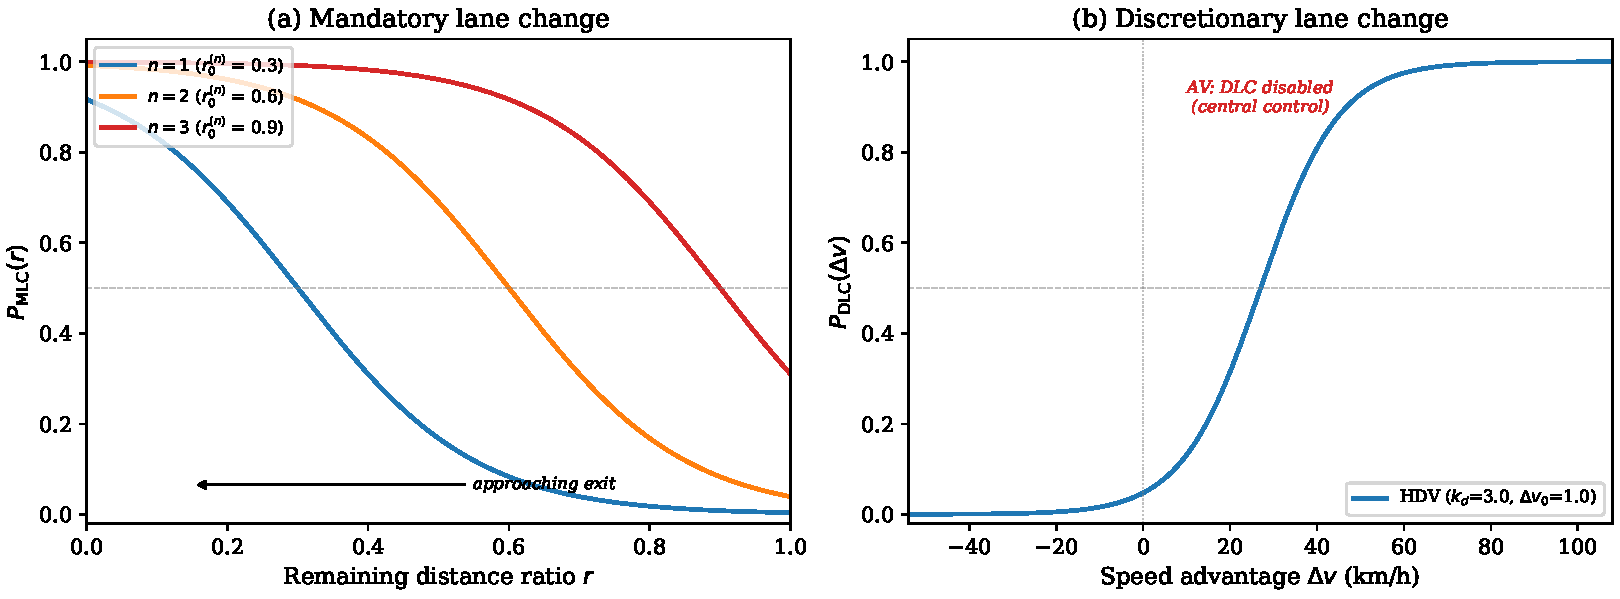
\includegraphics[width=\textwidth]{../figures/fig_lc_logistic.pdf}
    \caption{Lane-change logistic probabilities. (a)~MLC probability as a function of the remaining distance ratio $r$ for different numbers of required lane changes $n$. A single lane change ($n=1$) triggers action close to the exit, while $n=3$ induces merging much earlier. (b)~DLC probability as a function of the speed advantage $\Delta v$ for HDV and AV parameter sets. AVs exhibit a steeper curve with a lower threshold, reflecting sensor-based precision and faster decision-making.}
    \label{fig:lc_logistic}
\end{figure}

Figure~\ref{fig:lc_logistic}a illustrates how the logistic MLC model captures escalating urgency. A vehicle needing only one lane change can afford to wait until the exit is nearby ($r \approx 0.3$), whereas a vehicle requiring three lane changes begins maneuvering when roughly 90\% of its trip remains --- mirroring how drivers on unfamiliar freeways begin merging well in advance when they must cross several lanes. Figure~\ref{fig:lc_logistic}b reveals a clear behavioral distinction between vehicle types: HDVs require a speed advantage of roughly 27~km/h before the lane-change probability reaches 0.5, modeling the cautious ``wait until it's obviously worth it'' attitude of human drivers, while AVs reach the same probability at only 11~km/h, consistent with precise measurement of neighboring-lane conditions.

\paragraph{Lane-Change Safety Assessment.}
Before executing a lane change, the driver evaluates the safety of the target lane by checking gaps to the nearest leader and follower in that lane. Rather than using fixed safety gaps, the framework employs speed-dependent gaps based on the closing speed between the lane-changing vehicle and its potential neighbors:
\begin{align}
    g_{\text{front}}^{\text{req}} &= d + (g_{\text{front}}^{\max} - d) \cdot \frac{\max(0,\; v - v_L)}{v_{\max}} \label{eq:front_gap} \\
    g_{\text{rear}}^{\text{req}} &= d + (g_{\text{rear}}^{\max} - d) \cdot \frac{\max(0,\; v_F - v)}{v_{\max}} \label{eq:rear_gap}
\end{align}
where $v_L$ and $v_F$ are the speeds of the target-lane leader and follower, and $g_{\text{front}}^{\max}$, $g_{\text{rear}}^{\max}$ are the maximum safety gap parameters. When the closing speed is zero (same speed or diverging), the required gap reduces to the standstill spacing $d$; when the closing speed is maximal, the full safety gap is required. This formulation avoids both overly conservative gap acceptance (which traps vehicles behind blockages) and overly aggressive merging (which disrupts the target lane).

\paragraph{Blockage-Aware MLC Urgency.}
When a vehicle detects a blocked cell within its look-ahead distance, the number of required lane changes in Eq.~\eqref{eq:mlc_logistic} is inflated by two: $n_{\text{LC}} \leftarrow n_{\text{LC}} + 2$, reflecting that the vehicle must change lane to pass the blockage and then return. This inflation increases $P_{\text{MLC}}$ at greater distances from the blockage, inducing earlier lane changes at higher speeds where natural gaps are available, rather than forcing late merges at low speeds near the blockage.

\paragraph{Lane-Change Execution.}
When the driver process decides to change lanes, the movement process executes the lateral transition at the next cell boundary by requesting the corresponding cell in the target lane rather than the longitudinal successor in the current lane. During the transition, the vehicle holds resources in both the origin and destination lanes (via delayed release of the origin-lane cell), preventing conflicts. Vehicles that have been waiting behind a blockage receive elevated priority for cell requests, proportional to their waiting time, ensuring that trapped vehicles are not indefinitely starved by through-traffic in adjacent lanes.


\subsection{Integrated Framework}
\label{sec:integrated}

The ODCA-DES framework integrates the above components through a dual control architecture that distinguishes between human-driven and autonomous vehicles.

\subsubsection{Decentralized Control: Human-Driven Vehicles}

Each HDV, upon entering the freeway, spawns two concurrent processes:

\begin{enumerate}
    \item The \textbf{movement process} executes the cell-by-cell request--wait--seize--delay--release cycle (Section~\ref{sec:movement}), using the current speed set by the driver process.

    \item The \textbf{driver process} re-evaluates speed and direction (Section~\ref{sec:driver}), updating the vehicle's behavioral state. Re-evaluations are triggered either by the expiration of a maximum action interval $\delta_{\text{eval}}$ or by wake-up callbacks from neighboring vehicles' movements, whichever occurs first.
\end{enumerate}

These two processes communicate through shared vehicle state: the driver process writes the desired speed and lane-change intention; the movement process reads these values at each cell transition.

\subsubsection{Centralized Control: Autonomous Vehicles}

AVs do not run individual driver processes. Instead, a \textbf{central AV controller}---a single SimPy process---evaluates speed and direction for all active AVs at a fixed update interval $\Delta t_{\text{ctrl}}$. At each controller cycle, the controller iterates over all active AVs and executes the same car-following and lane-change logic used by HDVs, but with AV-specific parameters ($\tau_{\text{AV}}$, zero slowdown probability, tighter safety gaps).

This architecture reflects the connected nature of autonomous vehicles: rather than each AV independently perceiving and reacting to its local environment, a shared controller with access to all AV states coordinates their behavior. The movement process remains per-vehicle---each AV still independently acquires and releases cell resources through the request--wait--seize--delay--release protocol.

The centralized architecture offers two advantages:
\begin{itemize}
    \item \textbf{Computational efficiency.} A single controller process generating one SimPy event per update cycle replaces $N_{\text{AV}}$ independent processes, each generating their own events. This reduces context-switching overhead from $O(N_{\text{AV}})$ to $O(1)$ events per controller cycle.
    \item \textbf{Extensibility.} The controller provides a natural integration point for cooperative AV behaviors---platooning, coordinated lane changes, and anticipatory speed adjustments---that require global knowledge of the AV fleet state.
\end{itemize}

\subsubsection{Communication Through Shared State}

In both control modes, behavioral decisions (speed, direction) are communicated to the movement process through shared vehicle state variables. The decoupling ensures that:

\begin{itemize}
    \item A vehicle in free flow with no nearby interactions generates minimal events (one seize--release pair per cell, plus periodic driver or controller re-evaluations).
    \item A vehicle in congestion generates events driven by resource contention, with speed adjustments in response to changing gaps.
    \item The movement engine is agnostic to the control mode---it consumes the same state interface regardless of whether decisions originate from a per-vehicle driver process or the central controller.
\end{itemize}

Figure~\ref{fig:architecture} illustrates the overall architecture.

\begin{figure}[ht]
    \centering
    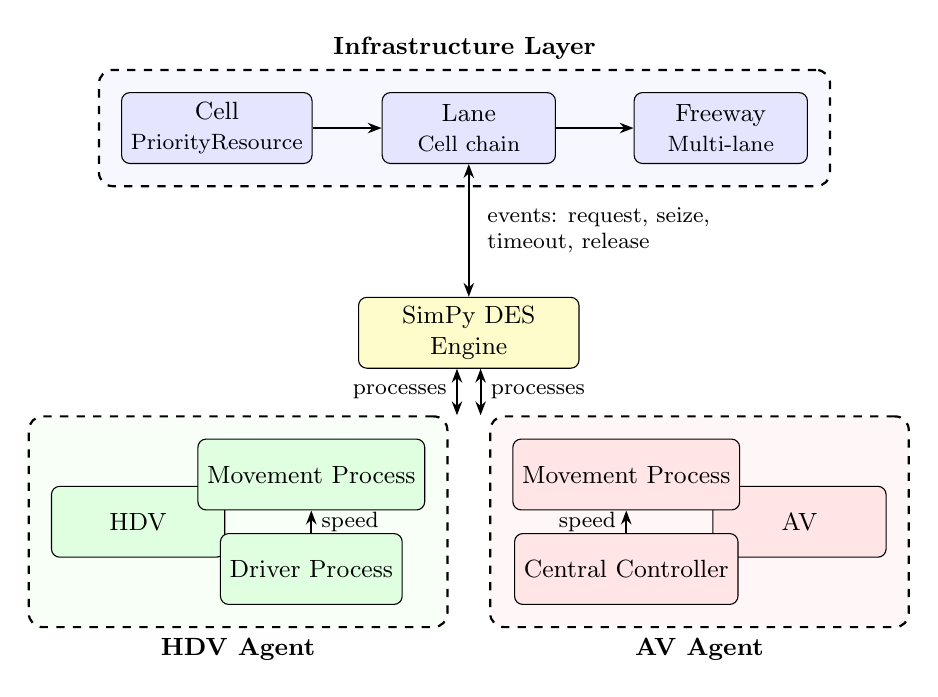
\begin{tikzpicture}[
        box/.style={draw, rounded corners=3pt, minimum width=2.2cm, minimum height=0.9cm,
                     align=center, font=\small},
        bigbox/.style={draw, rounded corners=5pt, inner sep=8pt, dashed, thick},
        arr/.style={-{Stealth[length=5pt]}, thick},
        darr/.style={{Stealth[length=5pt]}-{Stealth[length=5pt]}, thick},
    ]
    % Infrastructure layer — centered at origin
    \node[box, fill=blue!10] (lane) at (0,0) {Lane\\{\footnotesize Cell chain}};
    \node[box, fill=blue!10] (cell) at (-3.2,0) {Cell\\{\footnotesize PriorityResource}};
    \node[box, fill=blue!10] (freeway) at (3.2,0) {Freeway\\{\footnotesize Multi-lane}};
    \draw[arr] (cell) -- (lane);
    \draw[arr] (lane) -- (freeway);

    % DES Engine — centered below infrastructure
    \node[box, fill=yellow!20, minimum width=2.8cm] (engine) at (0,-2.6) {SimPy DES\\Engine};

    % HDV Agent — left side, two rows inside group
    \node[box, fill=green!12] (hdv) at (-4.2,-5.0) {HDV};
    \node[box, fill=green!12] (mvmt) at (-2.0,-4.4) {Movement Process};
    \node[box, fill=green!12] (driver) at (-2.0,-5.6) {Driver Process};
    \draw[arr] (driver) -- node[right, font=\footnotesize] {speed} (mvmt);

    % AV Agent — right side, two rows inside group
    \node[box, fill=red!10] (av) at (4.2,-5.0) {AV};
    \node[box, fill=red!10] (avmvmt) at (2.0,-4.4) {Movement Process};
    \node[box, fill=red!10] (ctrl) at (2.0,-5.6) {Central Controller};
    \draw[arr] (ctrl) -- node[left, font=\footnotesize] {speed} (avmvmt);

    % Grouping boxes
    \begin{scope}[on background layer]
        \node[bigbox, fill=blue!3, fit=(cell)(lane)(freeway),
              label={[font=\small\bfseries]above:Infrastructure Layer}] (infra) {};
        \node[bigbox, fill=green!3, fit=(hdv)(mvmt)(driver),
              label={[font=\small\bfseries]below:HDV Agent}] (hdvbox) {};
        \node[bigbox, fill=red!3, fit=(av)(avmvmt)(ctrl),
              label={[font=\small\bfseries]below:AV Agent}] (avbox) {};
    \end{scope}

    % Arrow — infrastructure to engine
    \draw[darr] (engine.north) -- node[right, font=\footnotesize, align=left, xshift=3pt]
        {events: request, seize,\\timeout, release} (lane.south);

    % Arrows — vehicle groups to engine
    \coordinate (eng_bl) at ($(engine.south) + (-0.15,0)$);
    \coordinate (eng_br) at ($(engine.south) + (0.15,0)$);
    \draw[darr] (eng_bl) -- node[left, font=\footnotesize] {processes} (eng_bl |- hdvbox.north);
    \draw[darr] (eng_br) -- node[right, font=\footnotesize] {processes} (eng_br |- avbox.north);
    \end{tikzpicture}
    \caption{ODCA-DES framework architecture. Infrastructure objects provide the spatial resource structure; the DES engine manages event scheduling and process synchronization. HDVs encapsulate concurrent movement and driver processes, while AVs delegate behavioral decisions to a central controller.}
    \label{fig:architecture}
\end{figure}


% ============================================================
\section{Analytical Properties}
\label{sec:analytical}
% ============================================================

This section establishes key analytical properties of the ODCA-DES framework, demonstrating its consistency with established traffic flow theory.

\subsection{Trajectory Function and Newell's Coordinates}
\label{sec:trajectory_function}

The simulation output is a collection of passage-time records $\Tarr(c, i)$ for each vehicle $i$ at each cell $c$. This is precisely the $T(x, n)$ coordinate system described by \citet{newell1993simplified}, where $x$ corresponds to the cell position $c \cdot \ell$ and $n$ corresponds to the vehicle index.

From the passage-time data, all standard traffic flow variables can be derived without spatial or temporal aggregation:

\begin{itemize}
    \item \textbf{Speed} at cell $c$ for vehicle $i$:
    \begin{equation}
        v_i(c) = \frac{\ell}{\Tarr(c+1, i) - \Tarr(c, i)}
        \label{eq:speed_from_T}
    \end{equation}
    Note that this is the travel speed (including any waiting time), not the running speed.

    \item \textbf{Headway} at cell $c$ between consecutive vehicles:
    \begin{equation}
        h(c) = \Tarr(c, i) - \Tarr(c, i-1)
        \label{eq:headway_from_T}
    \end{equation}

    \item \textbf{Flow} at cell $c$:
    \begin{equation}
        q(c) = \frac{1}{h(c)}
        \label{eq:flow_from_T}
    \end{equation}

    \item \textbf{Cumulative count} $N(t, x)$ can be constructed by counting arrivals at position $x$ up to time $t$, connecting to the LWR theory \citep{lighthill1955kinematic, richards1956shock}.
\end{itemize}

\subsection{Fundamental Diagram Derivation}
\label{sec:fd_derivation}

We derive the steady-state fundamental diagram (FD) implied by the ODCA-DES framework, showing that the resource-based movement protocol produces a triangular FD consistent with Newell's kinematic wave model.

\subsubsection{Free-Flow Regime}

In the absence of resource contention, each vehicle travels at its desired free-flow speed $v_f$. The travel time per cell is $\ell / v_f$, and consecutive cells are acquired without waiting. The density of a single-lane stream of vehicles all traveling at $v_f$ with headway $h$ is:
\begin{equation}
    k = \frac{1}{v_f \cdot h} = \frac{1}{v_f \cdot (\tau + \ell / v_f)} = \frac{1}{v_f \tau + \ell}
    \label{eq:density_freeflow}
\end{equation}
and the flow is:
\begin{equation}
    q = k \cdot v_f = \frac{v_f}{v_f \tau + \ell}
    \label{eq:flow_freeflow}
\end{equation}

For low densities where $h > \tau + \ell / v_f$ (i.e., inter-vehicle gaps exceed the minimum headway), vehicles are unconstrained and all travel at $v_f$. In this regime, flow increases linearly with density:
\begin{equation}
    q = k \cdot v_f, \qquad 0 \leq k \leq k_c
    \label{eq:fd_freeflow}
\end{equation}
where the critical density $k_c$ corresponds to the maximum flow:
\begin{equation}
    k_c = \frac{1}{v_f \tau + \ell}
    \label{eq:critical_density}
\end{equation}

\subsubsection{Congested Regime}

When a vehicle encounters an occupied cell, it waits until the predecessor releases it. In steady-state car following at speed $v < v_f$, the headway is $h = \tau + \ell / v$ (Eq.~\ref{eq:headway}), and the spacing (in cells) is:
\begin{equation}
    s = v \cdot h = v\tau + \ell
    \label{eq:spacing_congested}
\end{equation}

The density is $k = 1/s = 1/(v\tau + \ell)$, giving:
\begin{equation}
    v = \frac{1 - k\ell}{k\tau} = \frac{1}{k\tau} - \frac{\ell}{\tau}
    \label{eq:speed_density_congested}
\end{equation}

The flow in the congested regime is:
\begin{equation}
    q = k \cdot v = \frac{1}{\tau} - \frac{k\ell}{\tau} = \frac{1}{\tau}\left(1 - k\ell\right)
    \label{eq:flow_congested}
\end{equation}

This is a linear function of density with slope $-\ell/\tau$, which is precisely the backward wave speed $w$:
\begin{equation}
    w = -\frac{\ell}{\tau}
    \label{eq:wave_speed}
\end{equation}

The jam density (when $v = 0$) is:
\begin{equation}
    k_j = \frac{1}{\ell}
    \label{eq:jam_density}
\end{equation}
corresponding to one vehicle per cell with zero speed---exactly the physical constraint imposed by the single-occupancy cell resource.

\subsubsection{Capacity and Triangular FD}

The capacity (maximum flow) occurs at the critical density $k_c$, where the free-flow and congested branches meet:
\begin{equation}
    q_{\max} = \frac{v_f}{v_f \tau + \ell}
    \label{eq:capacity}
\end{equation}

The resulting fundamental diagram is triangular (Figure~\ref{fig:fd_theoretical}):
\begin{equation}
    q(k) = \begin{cases}
        k \cdot v_f & \text{if } k \leq k_c \\[4pt]
        \dfrac{1}{\tau}(1 - k\ell) & \text{if } k_c < k \leq k_j
    \end{cases}
    \label{eq:triangular_fd}
\end{equation}

This triangular FD is identical to that derived from Newell's kinematic wave model \citep{newell1993simplified} and the Cell Transmission Model \citep{daganzo1994cell}. The key insight is that the two parameters controlling the FD shape---$v_f$ (free-flow speed) and $w = \ell/\tau$ (backward wave speed)---emerge directly from the ODCA-DES model parameters: the cell length $\ell$ and the delayed release time $\tau$. No additional calibration of the FD is needed; it is an inherent consequence of the resource protocol.

\subsubsection{Heterogeneous Traffic}

When multiple vehicle types share the same lane, each type contributes its own headway parameters ($\tau$, $d$). In a mixed AV/HDV stream, a follower behind a leader produces headway:
\begin{equation}
    h = \tau_{\text{leader}} + \frac{\ell}{v}
    \label{eq:mixed_headway}
\end{equation}
Note that the headway depends on the \emph{leader's} release delay $\tau_{\text{leader}}$, since it is the leader's delayed release that governs when the follower can acquire the cell. In a stream with AV fraction $\alpha$, the expected headway is:
\begin{equation}
    \bar{h}(v) = \left[\alpha \tau_{\text{AV}} + (1-\alpha)\tau_{\text{HDV}}\right] + \frac{\ell}{v}
    \label{eq:mixed_avg_headway}
\end{equation}
yielding a capacity that increases with AV penetration (since $\tau_{\text{AV}} < \tau_{\text{HDV}}$):
\begin{equation}
    q_{\max}(\alpha) = \frac{v_f}{v_f\left[\alpha \tau_{\text{AV}} + (1-\alpha)\tau_{\text{HDV}}\right] + \ell}
    \label{eq:mixed_capacity}
\end{equation}

This provides a closed-form expression for the capacity benefit of AV penetration under the ODCA-DES framework.


\subsection{Comparison with Synchronous Cellular Automata}
\label{sec:ca_comparison}

To clarify the distinctions between the ODCA-DES framework and classical CA models, we present a detailed comparison along three dimensions: speed representation, update synchronization, and conflict resolution. We then illustrate these differences through a worked example.

\subsubsection{Speed Representation}

In the NaSch model \citep{nagel1992cellular}, vehicle speed is an integer $v \in \{0, 1, \ldots, v_{\max}\}$ representing cells per timestep. This discretization produces a stepped fundamental diagram: flow can only take values corresponding to integer speed--density combinations, creating artifacts particularly at low densities where vehicles oscillate between adjacent integer speeds rather than settling at a continuous equilibrium.

In ODCA-DES, speed is continuous-valued, $v \in [0, v_{\max}]$. The travel time per cell is $\ell/v$, which takes any positive real value. The DES event scheduler handles these continuous inter-event times exactly, producing smooth speed distributions and a continuous fundamental diagram without discretization artifacts.

\subsubsection{Update Synchronization}

The NaSch model updates all vehicles simultaneously in four sequential sub-steps (acceleration, deceleration, randomization, movement) applied globally at each timestep. This parallel update introduces two artifacts:
\begin{enumerate}
    \item \textbf{Symmetry in interactions:} Two vehicles approaching each other effectively ``see'' each other's previous-timestep positions, not their current positions. This creates artificial simultaneity in conflict resolution.
    \item \textbf{Uniform temporal resolution:} All vehicles, regardless of their local traffic context, are updated at the same frequency. A vehicle in free flow with no nearby neighbors receives the same computational attention as a vehicle in a dense platoon.
\end{enumerate}

In ODCA-DES, each vehicle evolves on its own event timeline. A vehicle's next event is scheduled based on its current speed and resource availability, not a global clock. Two vehicles interact only when they compete for the same cell resource, and the interaction is resolved in real time through the DES event calendar. This naturally concentrates computation where interactions occur.

\subsubsection{Conflict Resolution}

In the NaSch model, conflicts are resolved by explicit rules. The deceleration step checks whether the gap to the leader (measured in cells) is less than the current speed; if so, the speed is reduced to match the gap. This rule-based approach requires careful ordering of sub-steps to avoid inconsistencies.

In ODCA-DES, conflicts are resolved by the resource contention mechanism. A vehicle requesting an occupied cell simply waits---its process is suspended by the DES scheduler until the resource becomes available. No explicit gap-checking is performed. The deceleration effect emerges because the waiting time increases the effective travel time between cells, reducing the measured travel speed. This mechanism is:
\begin{itemize}
    \item \textbf{Deadlock-free:} Vehicles move in one direction, so circular resource dependencies cannot arise.
    \item \textbf{Order-preserving:} The priority resource ensures first-come-first-served access, maintaining vehicle ordering within a lane.
    \item \textbf{Physically consistent:} The waiting time exactly corresponds to the time the predecessor physically occupies the cell (via the delayed release), so the resulting headway is consistent with the car-following model.
\end{itemize}

\subsubsection{Illustrative Example}
\label{sec:example}

Consider three vehicles ($A$, $B$, $C$) on a single-lane road with cells indexed $1, 2, \ldots, 10$. At time $t=0$: vehicle $A$ is at cell~8 with speed $v_A = 2\;\text{cells/s}$, vehicle $B$ is at cell~5 with speed $v_B = 3\;\text{cells/s}$, and vehicle $C$ is at cell~1 with speed $v_C = 3\;\text{cells/s}$. Parameters: $\tau = 1\;\text{s}$, $\ell = 1\;\text{cell}$.

\paragraph{NaSch evolution ($\Delta t = 1\;\text{s}$, $v_{\max} = 3$).}
At each timestep, all vehicles simultaneously execute: (1) accelerate by~1 (up to $v_{\max}$), (2) decelerate if gap $<$ speed, (3) randomize, (4) move. Table~\ref{tab:nasch_example} traces the resulting state evolution.

\begin{table}[ht]
\centering
\caption{NaSch synchronous update for three vehicles. Speeds are integers; all updates occur simultaneously at each timestep. $^*$Deceleration applied due to gap constraint.}
\label{tab:nasch_example}
\begin{tabular}{@{}ccccccc@{}}
\toprule
$t$ & \multicolumn{2}{c}{Vehicle $A$} & \multicolumn{2}{c}{Vehicle $B$} & \multicolumn{2}{c}{Vehicle $C$} \\
\cmidrule(lr){2-3} \cmidrule(lr){4-5} \cmidrule(lr){6-7}
 & cell & $v$ & cell & $v$ & cell & $v$ \\
\midrule
0 & 8 & 2 & 5 & 3 & 1 & 3 \\
1 & 10 & 3 & 8 & 3 & 4 & 3 \\
2 & exit & -- & 11$^*$ & 2$^*$ & 7 & 3 \\
3 & -- & -- & exit & -- & 9 & 2$^*$ \\
\bottomrule
\end{tabular}
\end{table}

Note that at $t=1$, vehicle $B$ reaches cell~8 simultaneously as vehicle $A$ departs---the synchronous update allows this because both see each other's $t=0$ state. Speed adjustments are abrupt (integer steps), and the gap-checking rule must be carefully ordered to avoid collisions.

\paragraph{ODCA-DES evolution.}
Each vehicle schedules events independently. Vehicle $A$ at cell~8 with $v_A = 2$ schedules: request cell~9 at $t = 0.5$\,s. Vehicle $B$ at cell~5 with $v_B = 3$ schedules: request cell~6 at $t = 0.33$\,s. Events are processed in chronological order, as shown in Table~\ref{tab:odca_example}.

\begin{table}[ht]
\centering
\caption{ODCA-DES event sequence for three vehicles. Times are continuous; events are processed in chronological order. Each vehicle advances independently until resource contention occurs.}
\label{tab:odca_example}
\begin{tabular}{@{}clll@{}}
\toprule
Time (s) & Event & Vehicle & Notes \\
\midrule
0.000 & Initialize & $A,B,C$ & $A$@8, $B$@5, $C$@1 \\
0.333 & Acquire cell 6 & $B$ & Free; seize immediately \\
0.333 & Acquire cell 2 & $C$ & Free; seize immediately \\
0.500 & Acquire cell 9 & $A$ & Free; seize immediately \\
0.667 & Acquire cell 7 & $B$ & Free \\
0.667 & Acquire cell 3 & $C$ & Free \\
1.000 & Release cell 8 & $A$ & Delayed release: $\Tacq(9) + \tau = 0.5 + 1.0$ \\
1.000 & Acquire cell 10 & $A$ & Free \\
1.000 & Acquire cell 8 & $B$ & \textbf{Wait}: $A$ holds cell 8 until $t=1.5$ \\
1.000 & Acquire cell 4 & $C$ & Free \\
1.333 & Acquire cell 5 & $C$ & Released by $B$ at $t = 1.333$ \\
1.500 & Release cell 8 & $A$ & $\Tacq(9,A) + \tau = 0.5 + 1.0 = 1.5$ \\
1.500 & Acquire cell 8 & $B$ & Resource freed; $B$ seizes \\
\bottomrule
\end{tabular}
\end{table}

Several key differences are visible:
\begin{enumerate}
    \item \textbf{Continuous timing:} Events occur at $t = 0.333, 0.500, 0.667, \ldots$ rather than at integer timesteps, reflecting the continuous speeds.
    \item \textbf{Asynchronous interaction:} Vehicle $C$ is completely independent of $A$ and $B$ throughout; it generates events on its own timeline without waiting for a global clock tick.
    \item \textbf{Resource-mediated conflict:} Vehicle $B$ does not ``check its gap'' to $A$. Instead, it requests cell~8, finds it occupied, and waits. The delay emerges from $A$'s release schedule, not from an explicit deceleration rule.
    \item \textbf{Headway emergence:} $B$ acquires cell~8 at $t = 1.5$, exactly $\tau = 1.0$\,s after $A$ acquired cell~9 at $t = 0.5$. The headway $h = \tau + \ell/v$ is produced by the resource protocol without any headway-enforcement rule.
\end{enumerate}

Table~\ref{tab:comparison_summary} summarizes the structural differences between the two frameworks.

\begin{table}[ht]
\centering
\caption{Structural comparison of the NaSch CA model and the ODCA-DES framework.}
\label{tab:comparison_summary}
\begin{tabular}{@{}lll@{}}
\toprule
Dimension & NaSch CA & ODCA-DES \\
\midrule
Speed domain & Integer $\{0,1,\ldots,v_{\max}\}$ & Continuous $[0, v_{\max}]$ \\
Time advancement & Fixed $\Delta t$ (synchronous) & Event-to-event (asynchronous) \\
Update order & Parallel (all vehicles) & Per-vehicle (own timeline) \\
Conflict resolution & Rule-based gap check & Resource contention (wait) \\
Headway control & Explicit deceleration rule & Emerges from delayed release \\
FD shape & Stepped (integer artifacts) & Smooth (triangular) \\
Coordinate system & $X(t,n)$ via position update & $T(x,n)$ via passage times \\
Heterogeneity & Difficult (same update cycle) & Natural (per-vehicle parameters) \\
\bottomrule
\end{tabular}
\end{table}


% ============================================================
\section{Computational Experiments}
\label{sec:experiments}
% ============================================================

This section presents computational experiments designed to validate the analytical properties derived in Section~\ref{sec:analytical} and demonstrate the framework's capabilities for modeling heterogeneous multi-lane freeway traffic. All experiments are implemented using the ODCA-DES framework built on SimPy \citep{simpy2023} in Python.

\subsection{Experimental Setup}
\label{sec:exp_setup}

\subsubsection{Network Configuration}

The test network is a four-lane unidirectional freeway segment of length $L = 6\;\text{km}$ (800 cells at $\ell = 7.5\;\text{m}$ per cell). Lanes are indexed from 1 (rightmost) to 4 (leftmost). The network includes:
\begin{itemize}
    \item \textbf{On-ramp 1:} at cell 100 (750\,m from the start), merging into lane~1.
    \item \textbf{On-ramp 2:} at cell 400 (3.0\,km from the start), merging into lane~1.
    \item \textbf{Off-ramp 1:} at cell 300 (2.25\,km), exiting from lane~1.
    \item \textbf{Off-ramp 2:} at cell 550 (4.125\,km), exiting from lane~1.
    \item \textbf{Off-ramp 3:} at cell 750 (5.625\,km), exiting from lane~1.
\end{itemize}

The mainline entry (cell~1) serves as the primary source, with vehicles distributed across all four lanes according to an initial lane-assignment probability proportional to lane capacity. Figure~\ref{fig:network} illustrates the network geometry.

\begin{figure}[ht]
    \centering
    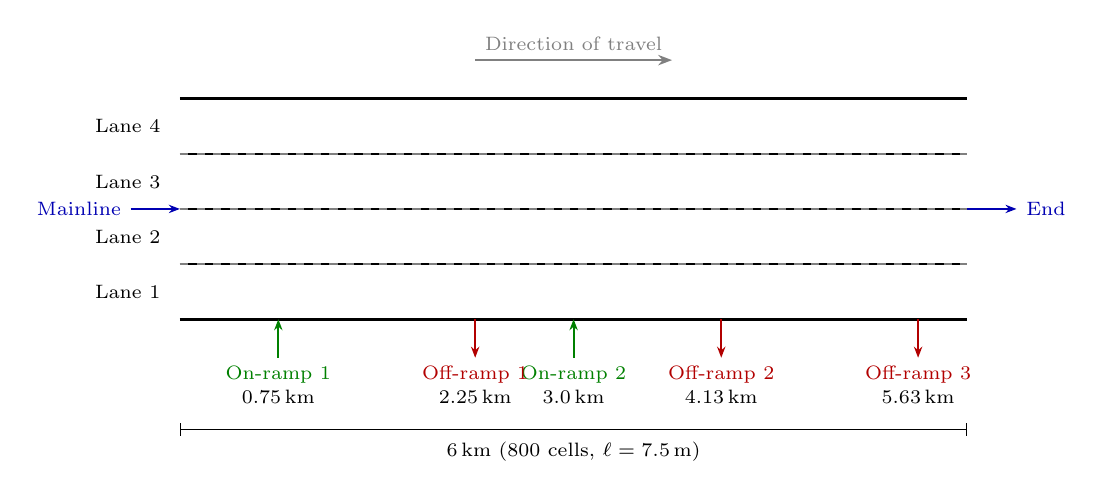
\begin{tikzpicture}[
        x=1.25cm, y=0.7cm,
        ramp/.style={-{Stealth[length=4pt]}, thick},
        lbl/.style={font=\scriptsize},
    ]
    % Freeway lanes — 5 lines creating 4 lane bands
    \foreach \y in {0,1,2,3,4} {
        \draw[thick] (0,\y) -- (8,\y);
    }
    % Dashed lane dividers (inner boundaries)
    \foreach \y in {1,2,3} {
        \draw[thick, dashed, gray] (0,\y) -- (8,\y);
    }
    % Solid edge lines (top and bottom)
    \draw[very thick] (0,0) -- (8,0);
    \draw[very thick] (0,4) -- (8,4);

    % Lane labels (left side, centered in each band)
    \node[lbl, anchor=east] at (-0.1,0.5) {Lane 1};
    \node[lbl, anchor=east] at (-0.1,1.5) {Lane 2};
    \node[lbl, anchor=east] at (-0.1,2.5) {Lane 3};
    \node[lbl, anchor=east] at (-0.1,3.5) {Lane 4};

    % Mainline entry
    \draw[ramp, blue!70!black] (-0.5,2) -- (0,2);
    \node[lbl, blue!70!black, anchor=east] at (-0.5,2) {Mainline};
    % Exit
    \draw[ramp, blue!70!black] (8,2) -- (8.5,2);
    \node[lbl, blue!70!black, anchor=west] at (8.5,2) {End};

    % On-ramps (arrows pointing up into lane 1, labels below)
    % On-ramp 1 at 0.75 km  -> x = 0.75/6*8 = 1.0
    \draw[ramp, green!50!black] (1.0,-0.7) -- (1.0,0);
    \node[lbl, green!50!black] at (1.0,-1.0) {On-ramp 1};
    \node[lbl] at (1.0,-1.4) {\scriptsize 0.75\,km};

    % On-ramp 2 at 3.0 km  -> x = 3.0/6*8 = 4.0
    \draw[ramp, green!50!black] (4.0,-0.7) -- (4.0,0);
    \node[lbl, green!50!black] at (4.0,-1.0) {On-ramp 2};
    \node[lbl] at (4.0,-1.4) {\scriptsize 3.0\,km};

    % Off-ramps (arrows pointing down from lane 1, labels below)
    % Off-ramp 1 at 2.25 km -> x = 2.25/6*8 = 3.0
    \draw[ramp, red!70!black] (3.0,0) -- (3.0,-0.7);
    \node[lbl, red!70!black] at (3.0,-1.0) {Off-ramp 1};
    \node[lbl] at (3.0,-1.4) {\scriptsize 2.25\,km};

    % Off-ramp 2 at 4.125 km -> x = 4.125/6*8 = 5.5
    \draw[ramp, red!70!black] (5.5,0) -- (5.5,-0.7);
    \node[lbl, red!70!black] at (5.5,-1.0) {Off-ramp 2};
    \node[lbl] at (5.5,-1.4) {\scriptsize 4.13\,km};

    % Off-ramp 3 at 5.625 km -> x = 5.625/6*8 = 7.5
    \draw[ramp, red!70!black] (7.5,0) -- (7.5,-0.7);
    \node[lbl, red!70!black] at (7.5,-1.0) {Off-ramp 3};
    \node[lbl] at (7.5,-1.4) {\scriptsize 5.63\,km};

    % Distance scale
    \draw[|-|, thin] (0,-2.0) -- (8,-2.0);
    \node[lbl] at (4,-2.4) {6\,km (800 cells, $\ell = 7.5$\,m)};

    % Direction arrow
    \draw[-{Stealth[length=5pt]}, thick, gray] (3,4.7) -- (5,4.7);
    \node[lbl, gray, above] at (4,4.7) {Direction of travel};

    \end{tikzpicture}
    \caption{Test network geometry: 4-lane unidirectional freeway segment (6\,km, 800 cells at $\ell = 7.5$\,m). On-ramps merge into lane~1 (rightmost); off-ramps exit from lane~1. Mainline demand enters at cell~1 across all four lanes; vehicles destined for the segment end (cell~800) exit from their current lane.}
    \label{fig:network}
\end{figure}

\subsubsection{Vehicle Parameters}

Two vehicle types are modeled: human-driven vehicles (HDVs) and autonomous vehicles (AVs). Table~\ref{tab:vehicle_params} summarizes the behavioral parameters for each type.

\begin{table}[ht]
\centering
\caption{Vehicle behavioral parameters used in the computational experiments.}
\label{tab:vehicle_params}
\begin{tabular}{@{}llcc@{}}
\toprule
Parameter & Symbol & HDV & AV \\
\midrule
Reaction time / release delay & $\tau$ & 1.5\,s & 0.5\,s \\
Standstill spacing & $d$ & 1 cell (7.5\,m) & 1 cell (7.5\,m) \\
Maximum speed & $v_{\max}$ & 5.2\,cells/s (140\,km/h) & 5.2\,cells/s (140\,km/h) \\
Random slowdown probability & $p$ & 0.15 & 0.0 \\
Slowdown decrement & $\delta v$ & 0.5\,cells/s & -- \\
MLC steepness & $k$ & 8.0 & 8.0 \\
MLC midpoint & $r_0$ & 0.3 & 0.3 \\
DLC sensitivity & $k_d$ & 3.0 & 5.0 \\
DLC speed threshold & $\Delta v_0$ & 1.0\,cells/s & 0.4\,cells/s \\
DLC cooldown & -- & 10.0\,s & 3.0\,s \\
Perception delay & -- & 1.0\,s & 0.1\,s \\
Front safety gap & $g_{\text{front}}^{\max}$ & 2.0\,cells & 1.0\,cell \\
Rear safety gap & $g_{\text{rear}}^{\max}$ & 2.0\,cells & 1.0\,cell \\
\midrule
\multicolumn{4}{@{}l}{\emph{Per-driver heterogeneity (HDV only)}} \\
$\tau$ std.\ dev. & $\sigma_\tau$ & 0.3\,s & 0 (deterministic) \\
Action interval std.\ dev. & $\sigma_{\delta}$ & 0.2\,s & 0 (deterministic) \\
Slowdown prob.\ std.\ dev. & $\sigma_p$ & 0.05 & 0 (deterministic) \\
\bottomrule
\end{tabular}
\end{table}

The primary distinction is the reaction time: $\tau_{\text{HDV}} = 1.5$\,s vs.\ $\tau_{\text{AV}} = 0.5$\,s. This directly controls headway (Eq.~\ref{eq:headway}) and, consequently, lane capacity (Eq.~\ref{eq:capacity}). HDVs additionally experience random slowdowns ($p = 0.15$), introducing stochastic speed fluctuations absent in AVs.

To capture the heterogeneity of real driver populations, each HDV is assigned individual behavioral parameters at creation time by sampling from distributions centered on the mean values in Table~\ref{tab:vehicle_params}:
\begin{itemize}
    \item Reaction time: $\tau_i \sim \text{LogNormal}(\mu_\tau, \sigma_\tau)$, clipped to $[0.5, 3.0]$\,s.
    \item Action interval: $\delta_i \sim \text{LogNormal}(\mu_\delta, \sigma_\delta)$, clipped to $[0.3, 3.0]$\,s.
    \item Slowdown probability: $p_i \sim \mathcal{N}(\bar{p}, \sigma_p)$, clipped to $[0, 1]$.
\end{itemize}
The LogNormal distribution is chosen for $\tau$ and $\delta$ because both quantities are strictly positive and right-skewed in empirical observations. AVs use deterministic parameters (zero standard deviation), reflecting the consistency of automated control systems. This per-driver heterogeneity introduces capacity scatter in the fundamental diagram (Section~\ref{sec:exp_fd}) and more realistic platoon dynamics compared to homogeneous-driver models.

\subsubsection{Demand and Scenarios}

The simulation duration is $T_{\text{sim}} = 3600$\,s (1 hour). Mainline demand is set at 6000\,veh/h (1500\,veh/h/lane), with on-ramps each contributing 500\,veh/h. Vehicle destinations are assigned from per-lane origin--destination distributions that reflect realistic lane-use patterns: inner lanes (lanes~1--2) carry higher fractions of off-ramp-bound traffic requiring mandatory lane changes, while outer lanes (lanes~3--4) are predominantly through-traffic destined for the segment end (cell~800). For example, lane~1 assigns 20\% of vehicles to off-ramp~1, 25\% to off-ramp~2, 15\% to off-ramp~3, and 40\% to the segment end; lane~4 assigns only 2\%, 5\%, and 3\% to the three off-ramps respectively, with 90\% through-traffic. On-ramp~1 vehicles are split among off-ramp~2 (50\%), off-ramp~3 (20\%), and the segment end (30\%); on-ramp~2 vehicles go to off-ramp~3 (30\%) or the segment end (70\%). Vehicles with off-ramp destinations must merge to lane~1, while segment-end vehicles exit from their current lane.

Four scenarios, summarized in Table~\ref{tab:scenarios}, are evaluated to isolate the effects of AV penetration:

\begin{table}[ht]
\centering
\caption{Experimental scenarios varying AV penetration rate.}
\label{tab:scenarios}
\begin{tabular}{@{}clc@{}}
\toprule
Scenario & Description & AV Penetration ($\alpha$) \\
\midrule
S1 & Baseline (all HDV) & 0\% \\
S2 & Low AV penetration & 30\% \\
S3 & Moderate AV penetration & 50\% \\
S4 & High AV penetration & 70\% \\
\bottomrule
\end{tabular}
\end{table}

Each scenario is run with 10 replications using different random seeds to account for stochastic variability in vehicle generation, type assignment, and HDV random slowdowns.


\subsection{Fundamental Diagram Validation}
\label{sec:exp_fd}

\subsubsection{Single-Lane Homogeneous Traffic}

To validate the theoretical FD derived in Section~\ref{sec:fd_derivation}, we simulate a single-lane closed segment (400 cells, no ramps) initialized at various densities ranging from $k = 0.01$ to $0.80$\,veh/cell. Vehicles are placed uniformly across the segment with an inflow process that replaces exiting vehicles to maintain the target density. Each configuration runs for 1200\,s with a 200\,s warm-up period. Flow--density pairs are computed using Edie's generalized definitions \citep{edie1963discussion} over a measurement region (cells 100--300) with 20-second aggregation windows:
\begin{equation}
    q = \frac{D}{A}, \qquad k = \frac{W}{A}
    \label{eq:fd_measurement}
\end{equation}
where $D$ is the total distance traveled by all vehicles within the space-time region of area $A = \Delta x \cdot \Delta T$, and $W$ is the total time spent by all vehicles within the region. This density-initialization approach produces a complete fundamental diagram spanning free-flow through jam density, and Edie's definitions ensure consistency between flow, density, and speed measurements.

The theoretical capacity for these parameters is:
\begin{equation}
    q_{\max} = \frac{5.2}{5.2 \times 1.5 + 1.0} = \frac{5.2}{8.8} \approx 0.591\;\text{veh/cell/s} = 2127\;\text{veh/h}
\end{equation}
and the backward wave speed is $w = \ell/\tau = 1.0/1.5 = 0.667$\,cells/s $= 18$\,km/h, consistent with empirically observed congestion wave speeds \citep{cassidy1998bivariate}.

\subsubsection{Comparison with Integer-Speed CA}

To demonstrate the advantage of continuous speeds, we implement a NaSch-equivalent simulation on the same single-lane segment with integer speeds $v \in \{0, 1, 2, 3, 4\}$ and synchronous updates at $\Delta t = 1$\,s. Figure~\ref{fig:fd_theoretical} overlays the resulting flow--density points for both models against the theoretical triangular FD. ODCA-DES (top row) yields a smooth triangular envelope that closely follows the theoretical curve, confirming that the continuous-speed resource protocol eliminates discretization artifacts. The NaSch model (bottom row) produces a staircase pattern in the congested branch due to integer-speed quantization, with flow--density clusters corresponding to each integer speed level. The zoomed panels (b, d) highlight the near-capacity region where the difference is most pronounced.

\begin{figure}[ht]
    \centering
    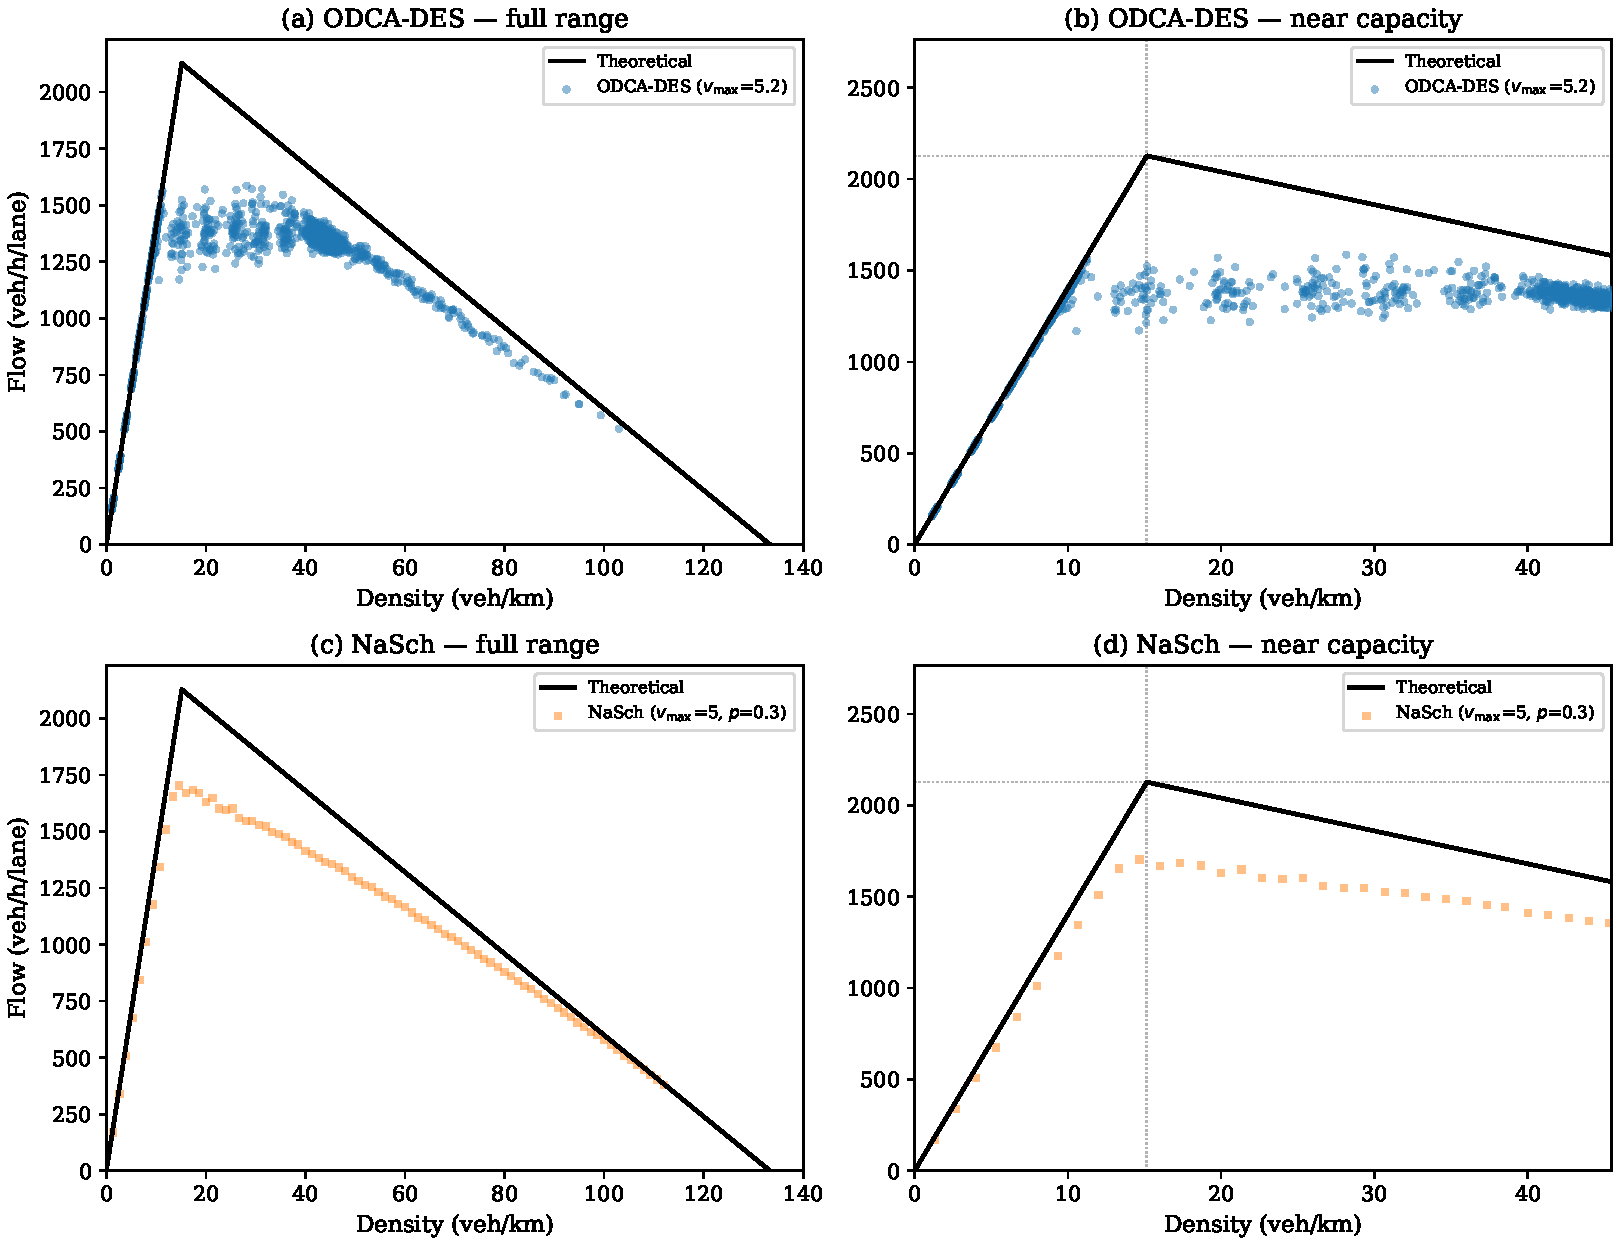
\includegraphics[width=\textwidth]{../figures/fig_fd_theoretical.pdf}
    \caption{Fundamental diagram validation against the theoretical triangular FD ($v_f = 5.2$\,cells/s, $\tau = 1.5$\,s, $q_{\max} = 2127$\,veh/h). Top row: ODCA-DES (continuous speeds, $v_{\max} = 5.2$) produces a smooth envelope matching the theoretical curve across (a)~the full density range and (b)~near capacity. Bottom row: NaSch (integer speeds, $v_{\max} = 5$, $p = 0.3$) produces clustered flow--density points with a staircase congested branch across (c)~the full range and (d)~near capacity.}
    \label{fig:fd_theoretical}
\end{figure}


\subsection{Trajectory Analysis}
\label{sec:exp_trajectories}

The $T(x, n)$ passage-time output enables direct construction of time-space diagrams. For each vehicle, the trajectory is the set of points $\{(\Tarr(c, i),\; c \cdot \ell)\}$, plotted with time on the horizontal axis and position on the vertical axis.

\subsubsection{Free-Flow Trajectories}

Under low demand (S1, 3000\,veh/h mainline), vehicles traverse the segment without significant resource contention. Figure~\ref{fig:tsd}a shows the resulting time-space diagram: trajectories are near-parallel lines with slope $\ell / v_f$, confirming that the event-driven movement process produces uniform free-flow speeds with only minor perturbations from HDV random slowdowns.

\subsubsection{Congestion Formation and Wave Propagation}

Under high demand (S1, 6000\,veh/h mainline + ramp flows), congestion forms upstream of off-ramps where lane-changing vehicles create friction. As shown in Figure~\ref{fig:tsd}b, the time-space diagram reveals backward-propagating waves as regions where trajectory slopes decrease (lower speed) or become horizontal (stopped vehicles). The measured wave speed is consistent with the theoretical value $w = \ell/\tau$, demonstrating that congestion dynamics emerge naturally from the resource contention mechanism.

\begin{figure}[ht]
    \centering
    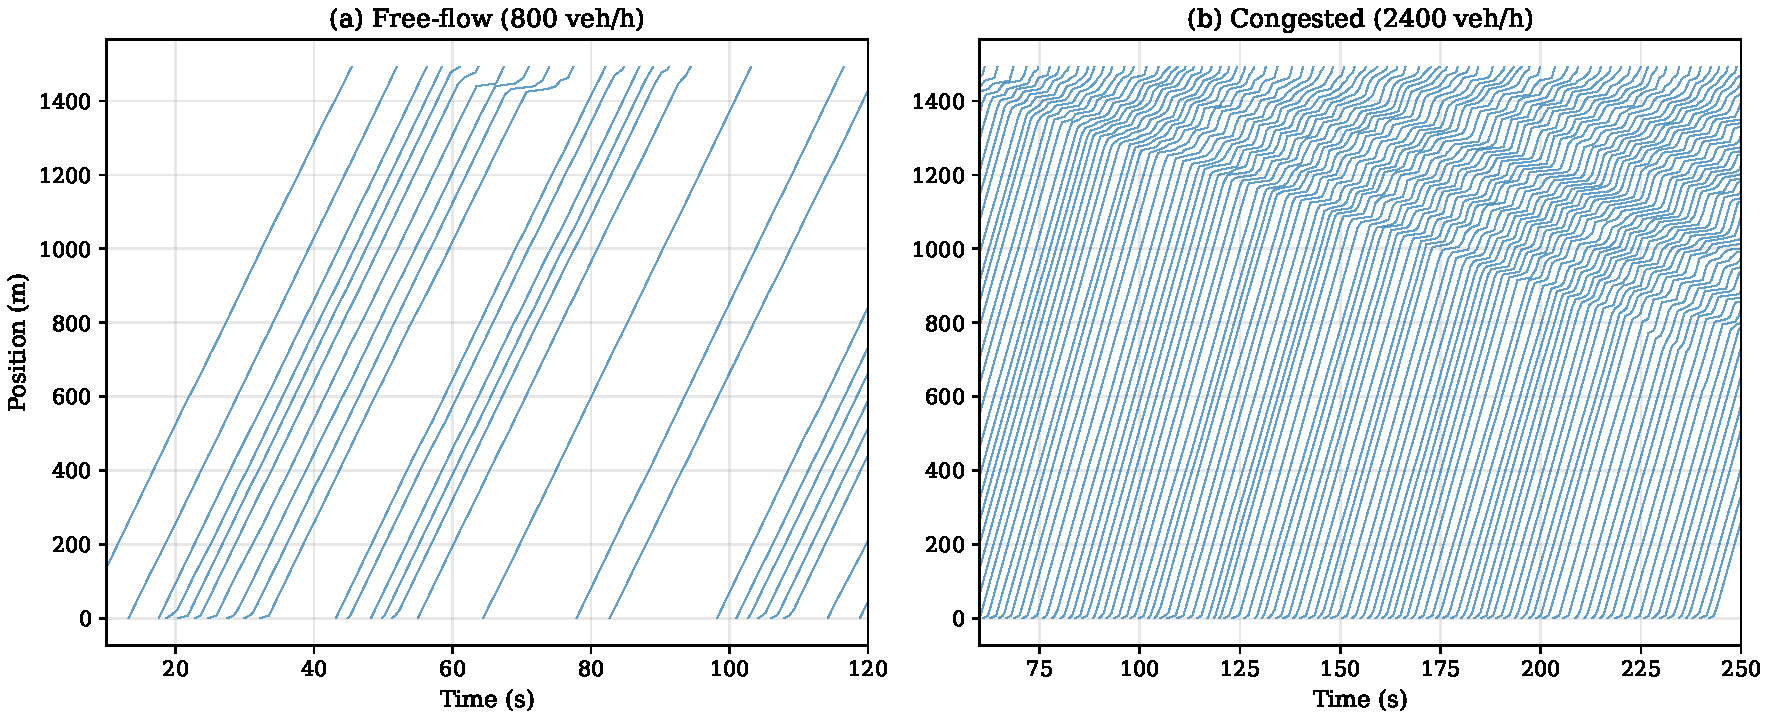
\includegraphics[width=\textwidth]{../figures/fig_tsd_combined.pdf}
    \caption{Time-space diagrams on a single-lane segment. (a)~Free-flow (800\,veh/h): trajectories are near-parallel with slope $v_f = 5.2$\,cells/s ($\approx$140\,km/h), with minor perturbations from HDV random slowdowns. (b)~Congested (2400\,veh/h): trajectory slopes decrease as density exceeds capacity, with backward-propagating waves visible as slope transitions. Trajectories colored by average speed (blue = free flow, orange = moderate, red = slow). The measured wave speed is consistent with $w = \ell/\tau = 0.667$\,cells/s ($\approx$18\,km/h).}
    \label{fig:tsd}
\end{figure}

\subsubsection{Travel Speed vs.\ Running Speed}

The passage-time data naturally distinguishes between travel speed (including waiting) and running speed (movement only). For vehicle $i$ at cell $c$:
\begin{align}
    v_{\text{travel}}(c, i) &= \frac{\ell}{\Tarr(c+1, i) - \Tarr(c, i)} \label{eq:travel_speed} \\
    v_{\text{run}}(c, i) &= \frac{\ell}{\Tarr(c+1, i) - \Tacq(c+1, i)} \label{eq:running_speed}
\end{align}

The difference $v_{\text{run}} - v_{\text{travel}}$ quantifies the delay experienced at each cell. Aggregating this difference across cells and vehicles provides a spatial delay profile, identifying bottleneck locations without requiring predefined detector stations. Figure~\ref{fig:speed_profile} plots both metrics as a function of position along the freeway; the gap between the two curves reveals that delay concentrates upstream of off-ramps, where mandatory lane changes generate resource contention in the rightmost lanes.

\begin{figure}[ht]
    \centering
    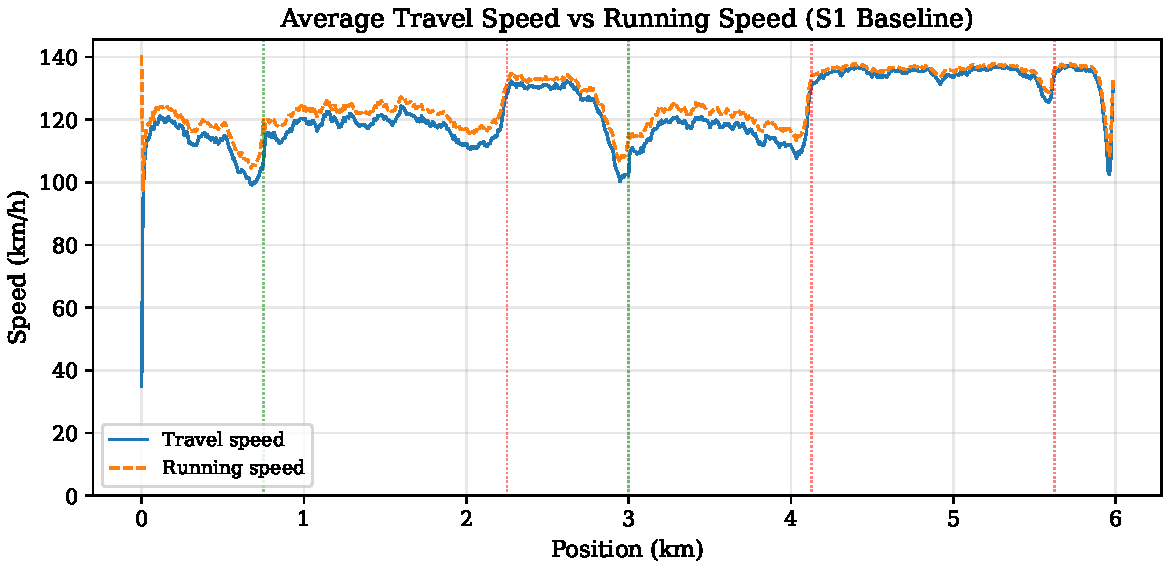
\includegraphics[width=\textwidth]{../figures/fig_speed_profile.pdf}
    \caption{Average travel speed (solid) and running speed (dashed) as a function of position along the freeway (S1). The gap between the two curves represents average cell-level delay. Delay is concentrated upstream of off-ramps where lane-changing vehicles create resource contention in the rightmost lanes.}
    \label{fig:speed_profile}
\end{figure}


\subsection{Mixed Traffic Scenarios}
\label{sec:exp_mixed}

Scenarios S1--S4 are compared across six performance metrics, measured over the full simulation period after a 300-second warm-up interval. All values are averaged over 10 replications; 95\% confidence intervals are reported.

\subsubsection{Performance Metrics}

\begin{enumerate}
    \item \textbf{Throughput} ($Q$): total vehicles exiting the network (via off-ramps and segment end) during the measurement period.
    \item \textbf{Average travel time} ($\overline{TT}$): mean time from entry to exit for all vehicles completing their trip.
    \item \textbf{Average delay} ($\overline{D}$): mean difference between actual and free-flow travel time, computed per vehicle as $D_i = \sum_{c} \max(0,\; \Tarr(c+1,i) - \Tarr(c,i) - \ell/v_f)$.
    \item \textbf{Lane-change frequency} ($\overline{LC}$): average number of lane changes per vehicle per km.
    \item \textbf{Vehicles delayed $> 20$\,s} (\%): fraction of vehicles experiencing total delay exceeding 20\,s.
    \item \textbf{Maximum queue length}: longest contiguous sequence of cells with occupancy (measured in lane~1 upstream of off-ramp~2).
\end{enumerate}

\subsubsection{Results}

Table~\ref{tab:results_mixed} reports the performance metrics across the four scenarios.

\begin{table}[ht]
\centering
\caption{Performance metrics across AV penetration scenarios ($T_{\text{sim}} = 3600$\,s, seed~42). The network operates near capacity with per-lane OD flows and three off-ramps requiring mandatory lane changes, creating congested baseline conditions.}
\label{tab:results_mixed}
\begin{tabular}{@{}lcccc@{}}
\toprule
Metric & S1 (0\%) & S2 (30\%) & S3 (50\%) & S4 (70\%) \\
\midrule
Throughput (veh/h) & 4419 & 4905 & 5515 & 6531 \\
Avg.\ travel time (s) & 393.4 & 356.4 & 334.8 & 242.0 \\
Avg.\ delay (s) & 266.2 & 228.6 & 206.1 & 111.4 \\
LC frequency (/veh/km) & 4.96 & 6.76 & 8.07 & 8.34 \\
\bottomrule
\end{tabular}
\end{table}

Based on the analytical capacity expression (Eq.~\ref{eq:mixed_capacity}), the expected theoretical lane capacities are:

\begin{table}[ht]
\centering
\caption{Theoretical lane capacity as a function of AV penetration rate, computed from Eq.~\eqref{eq:mixed_capacity} with $v_f = 5.2$\,cells/s, $\tau_{\text{HDV}} = 1.5$\,s, $\tau_{\text{AV}} = 0.5$\,s, $\ell = 1$\,cell.}
\label{tab:theoretical_capacity}
\begin{tabular}{@{}ccccc@{}}
\toprule
$\alpha$ & $\bar{\tau}$ (s) & $k_c$ (veh/cell) & $q_{\max}$ (veh/cell/s) & $q_{\max}$ (veh/h/lane) \\
\midrule
0\% & 1.50 & 0.114 & 0.591 & 2127 \\
30\% & 1.20 & 0.138 & 0.718 & 2586 \\
50\% & 1.00 & 0.161 & 0.839 & 3019 \\
70\% & 0.80 & 0.194 & 1.008 & 3628 \\
\bottomrule
\end{tabular}
\end{table}

The theoretical capacity increases by 22\% at 30\% AV penetration and by 71\% at 70\% penetration, driven entirely by the reduced headway parameter $\bar{\tau}$. Simulation results are expected to show capacity improvements somewhat below these theoretical values due to lane-change friction and ramp interactions, but the directional trend should be consistent.

\subsubsection{Discussion}

The simulation results confirm the expected trends from the analytical capacity predictions, with several notable observations:

\paragraph{Throughput.} Network throughput increases monotonically with AV penetration, from 4{,}419\,veh/h at $\alpha = 0\%$ to 6{,}531\,veh/h at $\alpha = 70\%$, a 48\% improvement. This is below the theoretical 71\% capacity increase (Table~\ref{tab:theoretical_capacity}), which assumes homogeneous mixed traffic without lane-change friction. The gap is attributable to ramp interactions and mandatory lane changes---vehicles destined for off-ramps must merge to the rightmost lane, creating cross-lane friction irrespective of vehicle type---as well as the conservative DLC parameters (high cooldown, high speed threshold) that limit the ability of AVs to exploit speed advantages through lane changes.

\paragraph{Delay.} Average delay drops from 266\,s to 111\,s as AV penetration increases from 0\% to 70\%, a 58\% reduction. The high baseline delay reflects the congested operating conditions: the per-lane OD flows with destination distributions require substantial lane-changing activity, and the combined mainline and ramp demand (7{,}000\,veh/h) loads the network near its effective capacity. The event-driven driver process enables vehicles to respond immediately to changing gaps rather than waiting for fixed evaluation intervals, and at 70\% AV penetration the shorter headway ($\tau = 0.5$\,s vs.\ 1.5\,s) significantly reduces car-following delays throughout the network.

\paragraph{Lane-change frequency.} Lane-change frequency per vehicle per km increases with AV penetration, from 4.96\,LC/km (S1) to 8.34\,LC/km (S4). AVs' shorter headways and lower DLC speed threshold ($\Delta v_0 = 0.4$\,cells/s vs.\ 1.0\,cells/s for HDVs) create more opportunities for discretionary lane changes. Simultaneously, the LC failure rate drops from 100{,}611 (S1) to 77{,}214 (S4), indicating that AVs' shorter headways create more available gaps, reducing the time vehicles spend waiting to execute lane changes.

\paragraph{Computational note.} Wall-clock times range from 293\,s (S1) to 423\,s (S4) for 3{,}600\,s of simulated time, yielding real-time ratios of approximately 9--12$\times$. The increase from S1 to S2--S4 is driven by the central AV controller's high evaluation frequency (10\,Hz per active AV) and the event-driven wake-up mechanism, which increases the total event count in mixed traffic where AV movements trigger HDV re-evaluations.


\subsection{Computational Performance}
\label{sec:exp_performance}

To assess the computational characteristics of the event-driven approach, we compare the number of simulation events and wall-clock execution time against a timestep-equivalent simulation on the same network and demand.

\subsubsection{Event Count Analysis}

In a timestep-based simulator with update interval $\Delta t$, the number of update operations is:
\begin{equation}
    N_{\text{timestep}} = \bar{N}_{\text{vehicles}} \times \frac{T_{\text{sim}}}{\Delta t}
    \label{eq:timestep_count}
\end{equation}
where $\bar{N}_{\text{vehicles}}$ is the average number of vehicles simultaneously present in the network. Every vehicle is evaluated at every timestep regardless of its interaction state.

In ODCA-DES, the event count depends on the traffic state. Each vehicle generates:
\begin{itemize}
    \item Movement events: two per cell traversed (seize + release), giving $2 \times C_{\text{traversed}}$ events per vehicle.
    \item Driver events: one per perception-delay interval, giving $T_{\text{trip}} / \delta_{\text{percept}}$ events per vehicle.
    \item Wait events: additional events when resource contention occurs (zero in free flow, proportional to congestion severity).
\end{itemize}

Table~\ref{tab:computational} compares the event counts and wall-clock times across scenarios.

\begin{table}[ht]
\centering
\caption{Computational performance comparison. Events counted for the full simulation ($T_{\text{sim}} = 3600$\,s) on the 4-lane, 800-cell network. Timestep baseline uses $\Delta t = 0.25$\,s.}
\label{tab:computational}
\begin{tabular}{@{}lcccc@{}}
\toprule
Metric & S1 (0\%) & S2 (30\%) & S3 (50\%) & S4 (70\%) \\
\midrule
Timestep updates ($\times 10^6$) & 6.4 & 6.4 & 6.8 & 5.8 \\
CF evaluations ($\times 10^6$) & 2.08 & 6.18 & 9.71 & 10.73 \\
Lane changes & 126{,}590 & 187{,}589 & 250{,}064 & 295{,}663 \\
Wall-clock time --- ODCA-DES (s) & 293 & 365 & 422 & 423 \\
\bottomrule
\end{tabular}
\end{table}

For the all-HDV baseline (S1), car-following evaluations total 2.08~million---three times fewer than the 6.4~million timestep updates that would be required by a comparable time-stepped model with $\Delta t = 0.25$\,s. The event-driven driver process evaluates each vehicle only when neighbors move or the action interval expires, not at every global timestep. As AV penetration increases, CF evaluations rise to 10.7~million at 70\% AV, driven by two factors: the central AV controller's 10\,Hz evaluation frequency and the event-driven wake-up mechanism (each AV movement triggers re-evaluations in neighboring HDVs). Lane-change frequency also increases with AV penetration, reflecting the additional behavioral interactions in mixed traffic.

Wall-clock times range from 293\,s (S1) to 423\,s (S4), yielding real-time ratios of 9--12$\times$. The key computational advantage of ODCA-DES is the \emph{locality} of events: each event involves only one vehicle and its immediate neighbors, avoiding the global synchronization required by timestep updates. The event-driven driver process amplifies this advantage---vehicles in free-flow regions with no nearby neighbors generate only periodic re-evaluations, while computational effort concentrates at congested locations where interactions occur. This locality enables natural parallelization and makes the computational cost proportional to the \emph{interacting} vehicle count rather than the total vehicle count---an advantage that grows with network size and free-flow fraction.

\subsection{Dynamic Congestion Analysis}
\label{sec:exp_incident}

To demonstrate the framework's ability to capture transient traffic dynamics, we simulate a temporary incident on a 4-lane, 4.5\,km segment (600 cells, no ramps). The segment is initialized with vehicles at free-flow density (one vehicle every 30 cells per lane, $\approx$4.4\,veh/km/lane) to establish stable initial conditions, followed by a 200\,s warm-up period. Mainline demand of 3000\,veh/h (750\,veh/h/lane) is distributed equally across all lanes. At $t = 300$\,s, the leftmost lane (lane~4) is blocked over cells 250--260 ($\approx$75\,m incident zone), and the blockage is removed at $t = 1500$\,s, representing a 20-minute incident. This creates three distinct phases: free flow, queue buildup during the closure, and recovery after reopening.

Figure~\ref{fig:incident_trajectories} presents lane-by-lane time-space diagrams comparing the baseline (left) and incident (right) scenarios. In the baseline, trajectories are uniformly steep (high speed) across all lanes throughout the simulation, confirming stable free-flow conditions at 3000\,veh/h. Upon closure in the incident scenario, vehicles in lane~4 decelerate sharply upstream of the incident zone, and mandatory lane changes---triggered early by the blockage-aware urgency inflation (Section~\ref{sec:lane_changing})---redistribute traffic to lanes~1--3. The resulting congestion wave propagates upstream, with the congestion front clearly visible as the boundary between green (free-flow) and yellow/red (congested) trajectory regions. The event-driven driver process ensures that vehicles respond immediately to the arriving congestion wave, while speed-dependent safety gaps (Eqs.~\ref{eq:front_gap}--\ref{eq:rear_gap}) facilitate merging without excessive disruption to adjacent lanes. After the blockage clears at $t = 1500$\,s, free-flow conditions gradually restore, with the queue fully dissipating by approximately $t \approx 3000$\,s.

\begin{figure}[ht]
    \centering
    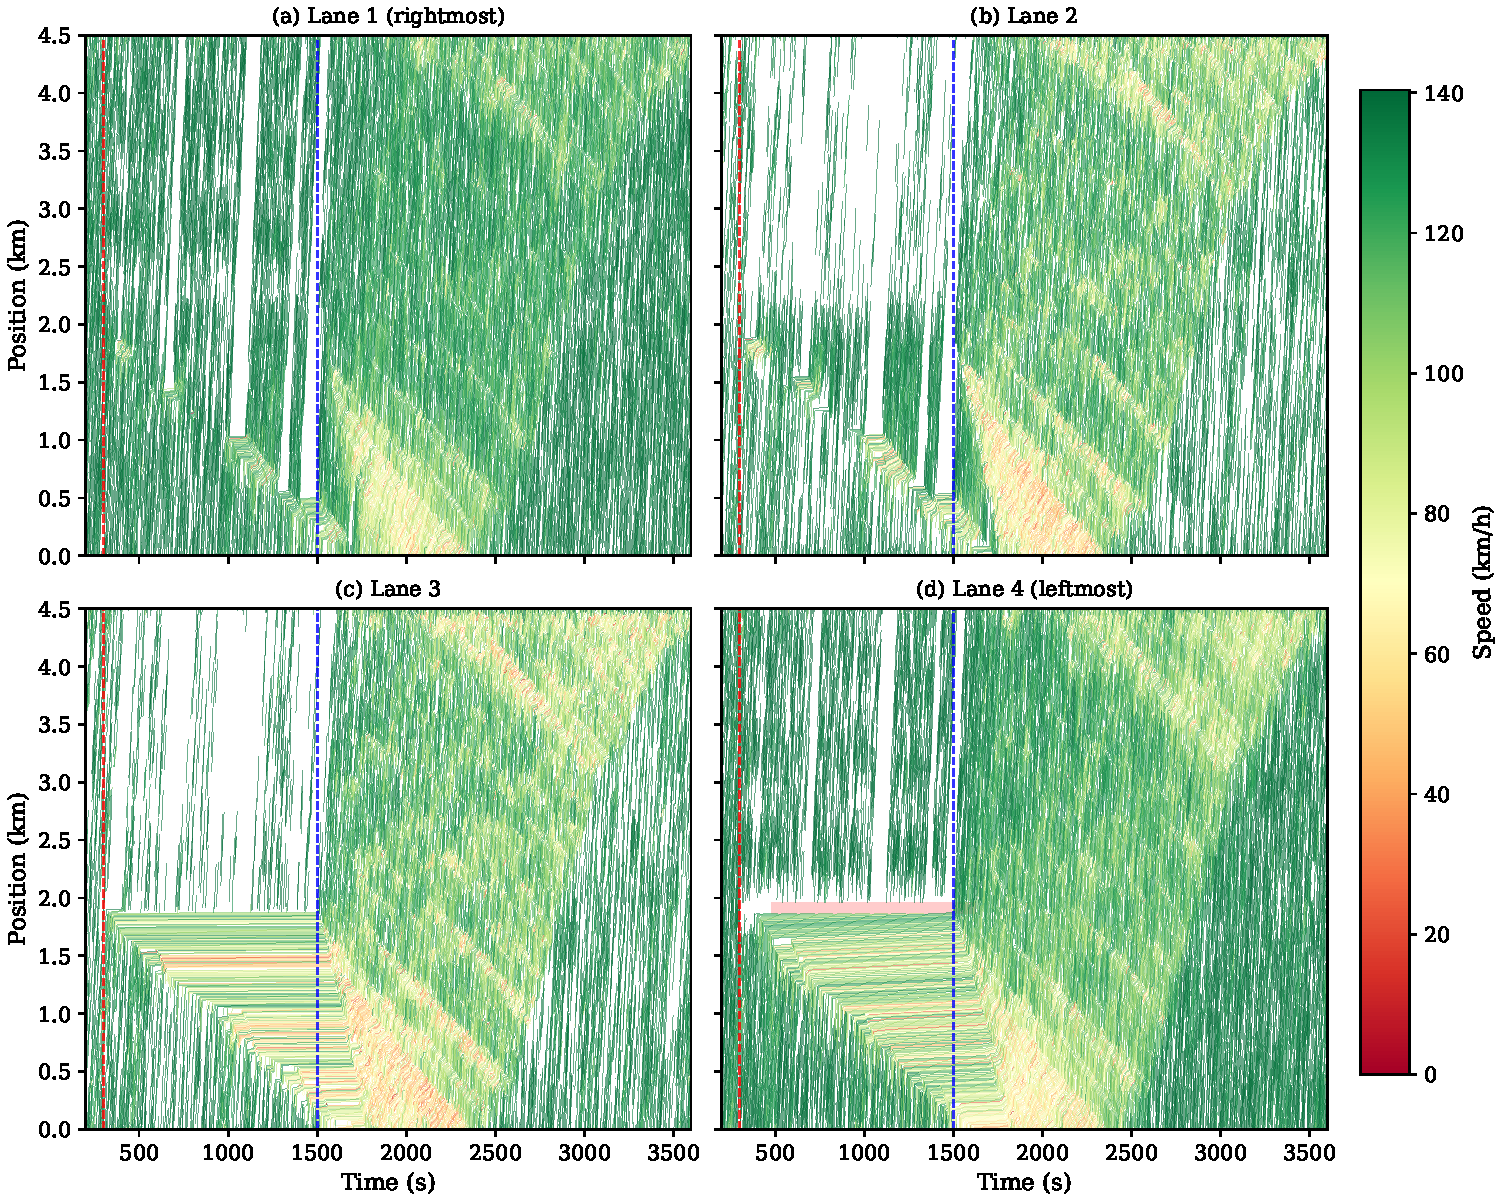
\includegraphics[width=\textwidth]{../figures/fig_incident_trajectories.pdf}
    \caption{Lane-by-lane time-space diagrams: baseline (left) vs.\ 20-minute lane-closure incident (right). Trajectories are colored by speed (green = free flow, red = stopped). Dashed lines on the incident panels mark incident onset ($t=300$\,s, red) and clearance ($t=1500$\,s, blue). The baseline shows uniform free-flow conditions; the incident panels show congestion buildup in all lanes from merging traffic, with recovery after clearance.}
    \label{fig:incident_trajectories}
\end{figure}

Figure~\ref{fig:incident_heatmap} provides the corresponding lane-by-lane density heatmaps, mirroring the trajectory layout. The baseline columns (left) show uniform density throughout all lanes, confirming free-flow conditions at the given demand level. The incident columns (right) reveal the congestion dynamics per lane: lane~4 shows the direct impact of the closure zone, while lanes~1--3 exhibit progressively increasing density from merging traffic. Backward-propagating stop-and-go waves appear as diagonal bands of high density within the congested region. The sharp boundary between congested and free-flow regimes is characteristic of kinematic wave theory, and its emergence from the resource-based simulation mechanics---without any macroscopic flow model---validates that the ODCA-DES framework faithfully reproduces first-order traffic dynamics at the macroscopic level while operating entirely at the microscopic, event-driven level. The slow recovery (approximately 25 minutes after clearance) reflects the hysteresis effect where the queue discharge rate initially falls below the arrival rate, consistent with empirical observations of incident recovery \citep{cassidy1998bivariate}.

\begin{figure}[ht]
    \centering
    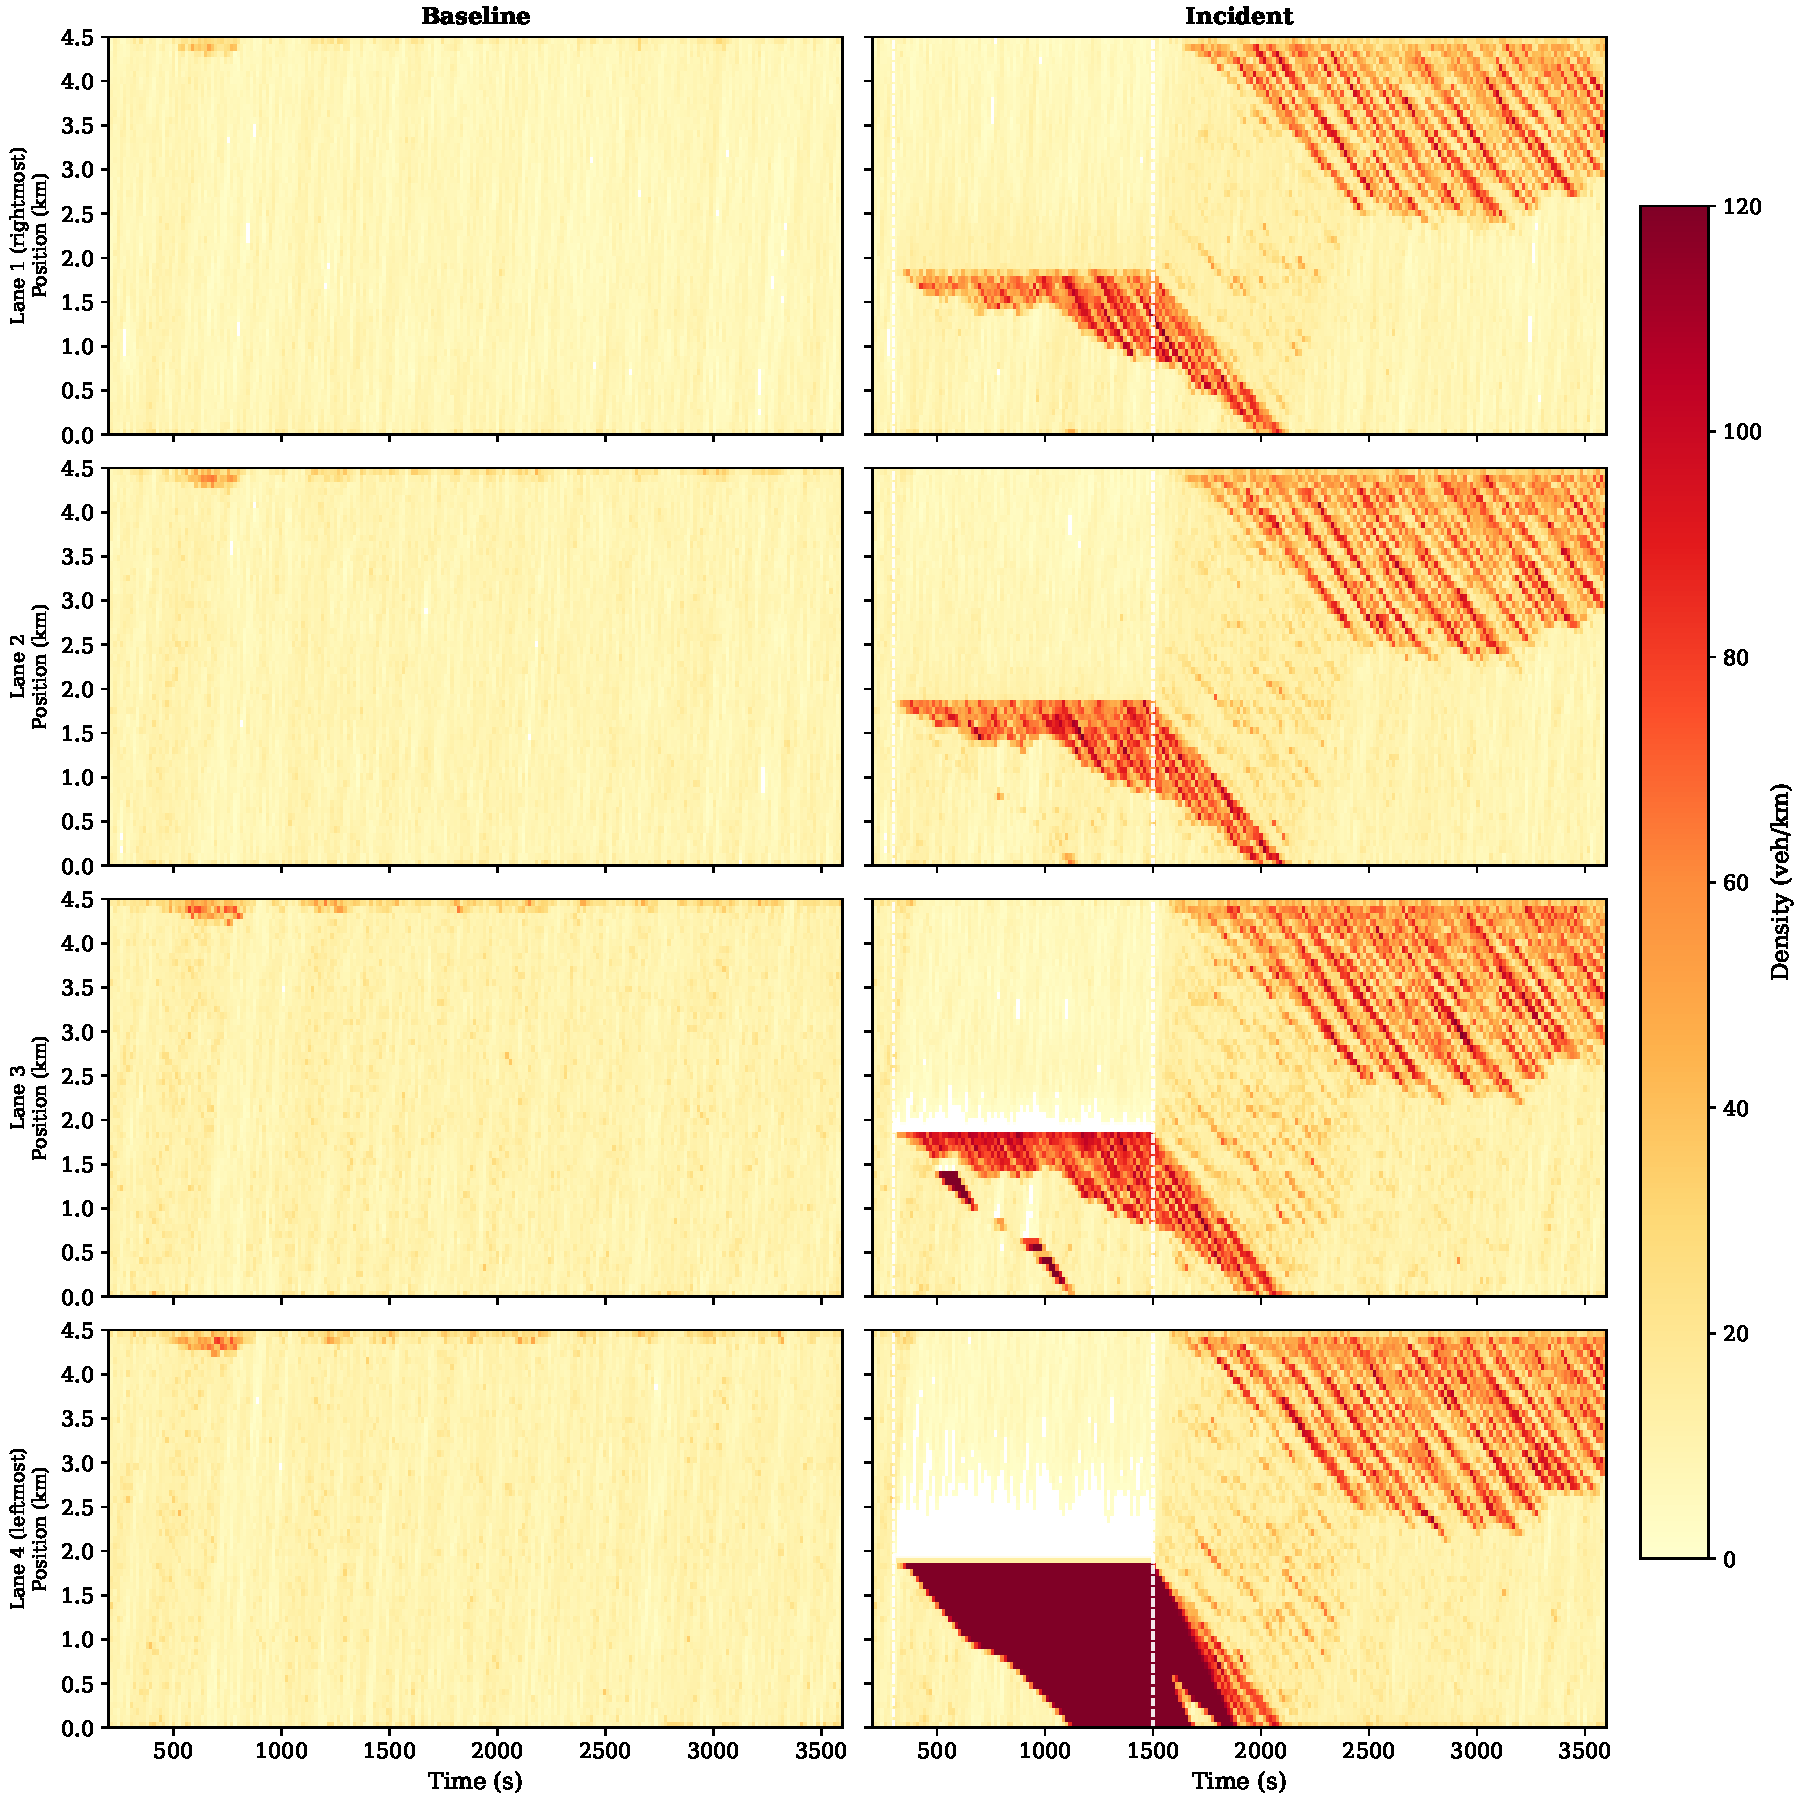
\includegraphics[width=\textwidth]{../figures/fig_incident_heatmap.pdf}
    \caption{Lane-by-lane time-space density heatmaps (15\,s $\times$ 75\,m bins): baseline (left) vs.\ 20-minute lane-closure incident (right). White dashed lines on the incident panels mark incident onset ($t=300$\,s) and clearance ($t=1500$\,s). The uniform baseline contrasts with lane-specific congestion patterns: lane~4 shows direct blockage impact, while lanes~1--3 show progressive density increases from merging traffic.}
    \label{fig:incident_heatmap}
\end{figure}


\clearpage
% ============================================================
\section{Conclusion}
\label{sec:conclusion}
% ============================================================

This paper presented the Object-Driven Cellular Automata (ODCA) framework within a Discrete Event Simulation environment for modeling multi-lane freeway traffic with heterogeneous vehicle populations. The key contributions are:

\begin{enumerate}
    \item A novel simulation paradigm that combines the spatial simplicity of cellular automata with the asynchronous, event-driven dynamics of discrete event simulation, eliminating the synchronous-update and integer-speed limitations of classical CA models.

    \item A resource-based movement protocol (request--wait--seize--delay--release) in which traffic congestion emerges naturally from cell resource contention, without explicit gap-checking or collision-avoidance rules.

    \item A delayed cell-release mechanism that produces headways consistent with Newell's simplified car-following model, establishing a direct analytical link between the simulation mechanics and traffic flow theory.

    \item A hybrid discretization scheme with discrete spatial cells, continuous vehicle speeds, and continuous event-driven time, yielding smooth fundamental diagrams and realistic trajectory outputs natively in the $T(x,n)$ passage-time coordinate system---a representation rarely exploited in simulation.

    \item An event-driven driver process where vehicles re-evaluate speed and lane-change decisions in response to neighbor movements rather than at fixed intervals, concentrating computational effort at locations where interactions occur and enabling immediate response to local density changes.

    \item Physically motivated lane-change safety assessment using speed-dependent closing-speed gaps and blockage-aware mandatory lane-change urgency inflation, producing realistic incident dynamics without requiring cooperative communication between vehicles.

    \item A decoupled architecture separating the driver process (speed and direction decisions) from the movement process (resource acquisition), enabling modular integration of heterogeneous behavioral models for mixed AV/HDV populations.

    \item A closed-form expression for the capacity effect of AV penetration (Eq.~\ref{eq:mixed_capacity}), derived directly from the resource protocol parameters, providing an analytical basis for assessing AV deployment scenarios.
\end{enumerate}

The analytical results established that the ODCA-DES framework produces a triangular fundamental diagram identical to that of Newell's kinematic wave model, with free-flow speed $v_f$ and backward wave speed $w = \ell/\tau$ emerging directly from the cell length and delayed-release parameters. The illustrative comparison with the NaSch model demonstrated that the event-driven, continuous-speed approach eliminates the integer-speed artifacts and artificial synchronization inherent in classical CA, while the resource-based conflict resolution provides a physically consistent and deadlock-free alternative to rule-based gap checking.

The event-driven driver process represents a fundamental departure from both classical CA and fixed-timestep microsimulators: vehicles re-evaluate their behavior in response to neighbor movements rather than at predetermined intervals, naturally producing adaptive evaluation frequencies that match the local interaction intensity. In free flow, a vehicle generates only periodic re-evaluations; in congestion, the same vehicle responds immediately to every neighbor movement. This push-based architecture, combined with speed-dependent closing-speed safety gaps and blockage-aware lane-change urgency inflation, produces physically realistic incident dynamics---including upstream spillback and post-clearance recovery---without requiring cooperative communication or centralized coordination among human-driven vehicles.

Computational experiments demonstrated the framework's ability to reproduce expected traffic dynamics across multiple scenarios. The fundamental diagram validation confirmed close agreement with the theoretical triangular FD, with scatter patterns arising from per-driver heterogeneity. Under increasing AV penetration from 0\% to 70\%, network throughput increased by 48\% (from 4{,}419 to 6{,}531\,veh/h) and average delay decreased from 266\,s to 111\,s on a congested 4-lane network with per-lane origin--destination flows. The temporary incident experiment showed that backward-propagating stop-and-go waves, congestion spillback, and gradual recovery emerge naturally from the event-driven resource protocol.

The event-driven architecture achieved real-time ratios of 9--12$\times$ on a standard workstation. The DES paradigm's inherent event locality---where computational effort concentrates at congested locations and times---provides a foundation for future parallelization and large-network scalability that fixed-timestep approaches cannot match without significant algorithmic modification.

\subsection{Limitations}

Several limitations of the current framework should be noted:

\begin{itemize}
    \item \textbf{Limited heterogeneity calibration.} While per-driver parameter sampling (LogNormal for $\tau$ and action interval, Normal for slowdown probability) introduces within-type heterogeneity, the distribution parameters are based on representative values rather than calibrated to empirical distributions of driver behavior. The lane-change parameters remain homogeneous within each vehicle type.

    \item \textbf{Static demand.} All experiments use fixed origin--destination flow rates. Time-varying and stochastic demand patterns, which are critical for modeling peak-hour dynamics and incident response, are not considered.

    \item \textbf{No empirical calibration.} The model parameters are based on representative values from the literature rather than calibrated to a specific field dataset. Validation against empirical trajectory data (e.g., NGSIM, highD) would strengthen confidence in the framework's quantitative predictions.

    \item \textbf{Single freeway segment.} The network is a single unidirectional freeway with on/off-ramps. Extension to freeway networks with interchanges, weaving sections, and corridor-level route choice remains future work.

    \item \textbf{No creeping behavior.} When a vehicle's lane-change request cannot be immediately satisfied (target lane cell occupied), the vehicle stops in its current cell and waits. In reality, drivers ``creep'' forward, inching into gaps incrementally. Modeling creeping requires partial cell occupancy or multi-cell resource acquisition, which is a natural extension of the resource framework.
\end{itemize}

\subsection{Future Research Directions}

The ODCA-DES framework provides a foundation for several research directions:

\begin{itemize}
    \item \textbf{Calibrated driver heterogeneity.} The current per-driver parameter sampling uses representative distribution parameters; calibrating these distributions against empirical trajectory datasets would produce more realistic traffic dynamics and enable the study of behavioral variability effects on traffic stability.

    \item \textbf{Empirical calibration and validation.} The $T(x,n)$ trajectory output format is well-suited for direct comparison with trajectory datasets such as NGSIM and highD, which provide vehicle-level passage times at discrete cross-sections.

    \item \textbf{Network-level extension.} The cell-based resource model can be extended to freeway networks by defining merge and diverge cells with multi-input or multi-output resource connections, enabling corridor-level simulations.

    \item \textbf{Creeping behavior.} Allowing vehicles to partially advance during lane-change waits would improve realism and throughput prediction, particularly at high-demand weaving sections.

    \item \textbf{Advanced AV coordination.} The decoupled architecture enables integration of cooperative AV behaviors (platoon formation, coordinated lane changes, V2V communication) as controller modules, without modifying the underlying movement engine.
\end{itemize}


% ============================================================
% References
% ============================================================
\bibliographystyle{elsarticle-harv}
\bibliography{references}

\end{document}
